\documentclass{exam} % Allows insertion of \question and generally looks nicer

%------------------------------------------------
%	            PACKAGES AND CONFIG
%------------------------------------------------
\usepackage{graphicx} % Required for inserting images
\usepackage{amsmath}
\usepackage{titling}
\usepackage{caption}
\usepackage{amsfonts}
\usepackage{amsthm}
\usepackage{hyperref}
\usepackage{algorithm}
\usepackage{algpseudocode}
\usepackage{tcolorbox} 
\usepackage[dutch]{babel}
\usepackage{tikz}
\usepackage{rotating} 
\usetikzlibrary{shapes, arrows}
\usetikzlibrary{positioning}

\counterwithin*{equation}{section}% Reset equation at \section
\counterwithin*{equation}{subsection}% Reset equation at \subsection
\counterwithin*{equation}{subsubsection}% Reset equation at \subsubsection
\setlength\parindent{0pt}
\hypersetup{
    colorlinks,
    citecolor=black,
    filecolor=black,
    linkcolor=black,
    urlcolor=black
}

%------------------------------------------------
%	                COMMANDS
%------------------------------------------------

\renewcommand\maketitlehooka{\null\mbox{}\vfill}
\renewcommand\maketitlehookd{\vfill\null}
\newcommand{\RomanNumeralCaps}[1]{\MakeUppercase{\romannumeral #1}}
\usepackage[framemethod=TikZ]{mdframed}

%------------------------------------------------
%                Proof Environment 
%------------------------------------------------

\newcounter{prf}[subsection]
\setcounter{prf}{0}

\renewcommand{\theprf}{\arabic{subsection}.\arabic{prf}}

\newenvironment{prf}[2][]{%
    \refstepcounter{prf}%
    \ifstrempty{#1}%
    {\mdfsetup{%
        frametitle={%
        \tikz[baseline=(current bounding box.east),outer sep=0pt]
        \node[anchor=east,rectangle,fill=red!20]
        {\strut Bewijs~\theprf};}}%
    }%
    {\mdfsetup{%
        frametitle={%
        \tikz[baseline=(current bounding box.east),outer sep=0pt]
        \node[anchor=east,rectangle,fill=red!20]
        {\strut Bewijs~\theprf:~#1};}}%
    }%
    \mdfsetup{innertopmargin=10pt,linecolor=red!20,%
    linewidth=2pt,topline=true,%
    frametitleaboveskip=\dimexpr-\ht\strutbox\relax
    }%
    \begin{mdframed}[]\relax%
    \label{#2}}{
        \vspace{-0.25cm}
        \begin{flushright}
            \qed % Move QED to the right
        \end{flushright}
        \vspace*{0cm}
        \end{mdframed}}

%------------------------------------------------
%              Theorem Environment 
%------------------------------------------------

\newcounter{theo}[subsection]
\setcounter{theo}{0}

\renewcommand{\thetheo}{\arabic{subsection}.\arabic{theo}}

\newenvironment{theo}[2][]{%
    \refstepcounter{theo}%
    \ifstrempty{#1}%
    {\mdfsetup{%
        frametitle={%
        \tikz[baseline=(current bounding box.east),outer sep=0pt]
        \node[anchor=east,rectangle,fill=cyan!20]
        {\strut Definitie~\thetheo};}}%
    }%
    {\mdfsetup{%
        frametitle={%
        \tikz[baseline=(current bounding box.east),outer sep=0pt]
        \node[anchor=east,rectangle,fill=cyan!20]
        {\strut Definitie~\thetheo:~#1};}}%
    }%
    \mdfsetup{innertopmargin=10pt,linecolor=cyan!20,%
    linewidth=2pt,topline=true,%
    frametitleaboveskip=\dimexpr-\ht\strutbox\relax
    }%
    \begin{mdframed}[]\relax%
    \label{#2}}{\vspace{0.25cm}\end{mdframed}}

%------------------------------------------------
%                Lemma Environment 
%------------------------------------------------

\newcounter{lem}[subsection]
\setcounter{lem}{0}

\renewcommand{\thelem}{\arabic{subsection}.\arabic{lem}}

\newenvironment{lem}[2][]{%
    \refstepcounter{lem}%
    \ifstrempty{#1}%
    {\mdfsetup{%
        frametitle={%
        \tikz[baseline=(current bounding box.east),outer sep=0pt]
        \node[anchor=east,rectangle,fill=green!20]
        {\strut Lemma~\thelem};}}%
    }%
    {\mdfsetup{%
        frametitle={%
        \tikz[baseline=(current bounding box.east),outer sep=0pt]
        \node[anchor=east,rectangle,fill=green!20]
        {\strut Lemma~\thelem:~#1};}}%
    }%
    \mdfsetup{innertopmargin=10pt,linecolor=green!20,%
    linewidth=2pt,topline=true,%
    frametitleaboveskip=\dimexpr-\ht\strutbox\relax
    }%
    \begin{mdframed}[]\relax%
    \label{#2}}{\vspace{0.25cm}\end{mdframed}}

%------------------------------------------------
%              Example Environment
%------------------------------------------------

\newcounter{ex}[subsection]
\setcounter{ex}{0}

\renewcommand{\theex}{\arabic{subsection}.\arabic{ex}}

\newenvironment{ex}[2][]{%
    \refstepcounter{ex}%
    \ifstrempty{#1}%
    {\mdfsetup{%
        frametitle={%
        \tikz[baseline=(current bounding box.east),outer sep=0pt]
        \node[anchor=east,rectangle,fill=orange!20]
        {\strut Voorbeeld~\theex};}}%
    }%
    {\mdfsetup{%
        frametitle={%
        \tikz[baseline=(current bounding box.east),outer sep=0pt]
        \node[anchor=east,rectangle,fill=orange!20]
        {\strut Voorbeeld~\theex:~#1};}}%
    }%
    \mdfsetup{innertopmargin=10pt,linecolor=orange!20,%
    linewidth=2pt,topline=true,%
    frametitleaboveskip=\dimexpr-\ht\strutbox\relax
    }%
    \begin{mdframed}[]\relax%
    \label{#2}}{\vspace{0.25cm}\end{mdframed}}

%------------------------------------------------
%               Property Environment 
%------------------------------------------------

\newcounter{pro}[subsection]
\setcounter{pro}{0}

\renewcommand{\thepro}{\arabic{subsection}.\arabic{pro}}

\newenvironment{pro}[2][]{%
    \refstepcounter{pro}%
    \ifstrempty{#1}%
    {\mdfsetup{%
        frametitle={%
        \tikz[baseline=(current bounding box.east),outer sep=0pt]
        \node[anchor=east,rectangle,fill=purple!20]
        {\strut Eigenschap~\thepro};}}%
    }%
    {\mdfsetup{%
        frametitle={%
        \tikz[baseline=(current bounding box.east),outer sep=0pt]
        \node[anchor=east,rectangle,fill=purple!20]
        {\strut Eigenschap~\thepro:~#1};}}%
    }%
    \mdfsetup{innertopmargin=10pt,linecolor=purple!20,%
    linewidth=2pt,topline=true,%
    frametitleaboveskip=\dimexpr-\ht\strutbox\relax
    }%
    \begin{mdframed}[]\relax%
    \label{#2}}{\vspace{0.25cm}\end{mdframed}}

%------------------------------------------------
%             Application Environment
%------------------------------------------------

\newcounter{app}[subsection]
\setcounter{app}{0}

\renewcommand{\theapp}{\arabic{subsection}.\arabic{app}}

\newenvironment{app}[2][]{%
    \refstepcounter{app}%
    \ifstrempty{#1}%
    {\mdfsetup{%
        frametitle={%
        \tikz[baseline=(current bounding box.east),outer sep=0pt]
        \node[anchor=east,rectangle,fill=magenta!20]
        {\strut Toepassing~\theapp};}}%
    }%
    {\mdfsetup{%
        frametitle={%
        \tikz[baseline=(current bounding box.east),outer sep=0pt]
        \node[anchor=east,rectangle,fill=magenta!20]
        {\strut Toepassing~\theapp:~#1};}}%
    }%
    \mdfsetup{innertopmargin=10pt,linecolor=magenta!20,%
    linewidth=2pt,topline=true,%
    frametitleaboveskip=\dimexpr-\ht\strutbox\relax
    }%
    \begin{mdframed}[]\relax%
    \label{#2}}{\vspace{0.25cm}\end{mdframed}}

%------------------------------------------------
%               Summary Environment
%------------------------------------------------

\newcounter{summ}[subsection]
\setcounter{summ}{0}

\renewcommand{\thesumm}{\arabic{subsection}.\arabic{summ}}

\newenvironment{summ}[2][]{%
    \refstepcounter{summ}%
    \ifstrempty{#1}%
    {\mdfsetup{%
        frametitle={%
        \tikz[baseline=(current bounding box.east),outer sep=0pt]
        \node[anchor=east,rectangle,fill=violet!20]
        {\strut Samenvatting~\thesumm};}}%
    }%
    {\mdfsetup{%
        frametitle={%
        \tikz[baseline=(current bounding box.east),outer sep=0pt]
        \node[anchor=east,rectangle,fill=violet!20]
        {\strut Samenvatting~\thesumm:~#1};}}%
    }%
    \mdfsetup{innertopmargin=10pt,linecolor=violet!20,%
    linewidth=2pt,topline=true,%
    frametitleaboveskip=\dimexpr-\ht\strutbox\relax
    }%
    \begin{mdframed}[]\relax%
    \label{#2}}{\vspace{0.25cm}\end{mdframed}}

%------------------------------------------------
%             Comparison Environment
%------------------------------------------------

\newcounter{vrg}[subsection]
\setcounter{vrg}{0}

\renewcommand{\thevrg}{\arabic{subsection}.\arabic{vrg}}

\newenvironment{vrg}[2][]{%
    \refstepcounter{vrg}%
    \ifstrempty{#1}%
    {\mdfsetup{%
        frametitle={%
        \tikz[baseline=(current bounding box.east),outer sep=0pt]
        \node[anchor=east,rectangle,fill=teal!20]
        {\strut Vergelijking~\thevrg};}}%
    }%
    {\mdfsetup{%
        frametitle={%
        \tikz[baseline=(current bounding box.east),outer sep=0pt]
        \node[anchor=east,rectangle,fill=teal!20]
        {\strut Vergelijking~\thevrg:~#1};}}%
    }%
    \mdfsetup{innertopmargin=10pt,linecolor=teal!20,%
    linewidth=2pt,topline=true,%
    frametitleaboveskip=\dimexpr-\ht\strutbox\relax
    }%
    \begin{mdframed}[]\relax%
    \label{#2}}{\vspace{0.25cm}\end{mdframed}}

%------------------------------------------------
%               Algorithm Environment
%------------------------------------------------

\newcounter{alg}[subsection]
\setcounter{alg}{0}

\renewcommand{\thealg}{\arabic{subsection}.\arabic{alg}}

\newenvironment{alg}[2][]{%
    \refstepcounter{alg}%
    \ifstrempty{#1}%
    {\mdfsetup{%
        frametitle={%
        \tikz[baseline=(current bounding box.east),outer sep=0pt]
        \node[anchor=east,rectangle,fill=violet!20]
        {\strut Algoritme~\thealg};}}%
    }%
    {\mdfsetup{%
        frametitle={%
        \tikz[baseline=(current bounding box.east),outer sep=0pt]
        \node[anchor=east,rectangle,fill=violet!20]
        {\strut Algoritme~\thealg:~#1};}}%
    }%
    \mdfsetup{innertopmargin=10pt,linecolor=violet!20,%
    linewidth=2pt,topline=true,%
    frametitleaboveskip=\dimexpr-\ht\strutbox\relax
    }%
    \begin{mdframed}[]\relax%
    \label{#2}}{\vspace{0.25cm}\end{mdframed}}


% Custom subsection numbering
\renewcommand{\thesubsection}{\arabic{subsection}}

% Command to add unnumbered sections to ToC
\newcommand{\sectionWithToC}[1]{
    \section*{#1} % Unnumbered section
    \addcontentsline{toc}{section}{#1} % Add it to ToC
}

% Custom intro page without section numbering
\newcommand{\introPage}[1]{
    \vspace*{\fill}
    \begin{center}
        \sectionWithToC{#1}
    \end{center}
    \vspace*{\fill}
}


%------------------------------------------------
%	            START OF DOCUMENT
%------------------------------------------------

\title{Numerieke Benadering}
\author{Pieter Vanderschueren}
\date{Academiejaar 2024-2025}

\begin{document}

\begin{titlingpage}
\maketitle
\end{titlingpage}

\newpage

%------------------------------------------------
%	              INTRODUCTION
%------------------------------------------------

% \introPage{Inleiding}

%------------------------------------------------
%	           TABLE OF CONTENTS
%------------------------------------------------

\newpage

\tableofcontents

\newpage

%------------------------------------------------
%	       LINEAIRE BENADERINGSPROBLEMEN
%------------------------------------------------

\introPage{Lineaire Benaderingsproblemen}

\newpage

\subsection{Benadering van vectoren}

\vspace{0.5cm}

\subsubsection{Terminologie}

\vspace{0.5cm}

\begin{theo}[Orthogonale en orthonormale basissen]{theo:orthogonale_orthonormale_basissen}
    We spreken van een orthogonale, respectievelijk orthonormale basis als de basisvectoren $\{a_1, \ldots, a_n\}$ orthogonaal, respectievelijk orthonormaal zijn. Als een basis niet orthogonaal is, spreken we van een scheve basis.
\end{theo}

\begin{theo}[Grammatrix]{theo:grammatrix}
    Voor een basis $\{a_1, \ldots, a_n\}$ van deelruimte $\mathcal{D}$ en twee vectoren $v, w \in \mathcal{D}$ ontbonden als
    \begin{equation*}
            v = \sum_{i=1}^{n} \alpha_i a_i, \
            w = \sum_{i=1}^{n} \beta_i a_i
    \end{equation*}
    geldt dat het inwendig product ($\langle v, w \rangle = v^*w$) van $v$ en $w$ gelijk is aan
    \begin{align*}
        \langle v, w \rangle 
            = \left( \sum_{i=1}^{n} \alpha_i a_i^* \right)\left( \sum_{i=1}^{n} \beta_i a_i \right) 
            = 
                \begin{bmatrix} \alpha_1 & \cdots & \alpha_n \end{bmatrix} 
                \underbrace{\begin{bmatrix} \langle a_1, a_1 \rangle & \cdots & \langle a_1, a_n \rangle \\ \vdots & \ddots & \vdots \\ \langle a_n, a_1 \rangle & \cdots & \langle a_n, a_n \rangle \end{bmatrix}}_{G} 
                \begin{bmatrix} \beta_1 \\ \vdots \\ \beta_n \end{bmatrix}
    \end{align*}
    waarbij deze G de zogenaamde grammatrix is horende bij de basis $\{a_1, \ldots, a_n\}$.
\end{theo}

\begin{pro}[Grammatrix]{pro:grammatrix}
    \begin{itemize}
        \item Is de basis orthogonaal, dan is de grammatrix diagonaal.
        \item Is de basis orthonormaal, dan is de grammatrix de eenheidsmatrix.
    \end{itemize}
\end{pro}

\begin{theo}[Projector]{theo:projector}
    Een projector is een matrix $P \in \mathbb{C}^{m \times m}$ die idempotent is, dit is $P^2 = P$. De meetkundige betekenis is als volgt. Matrix $P$ projecteert een vector op de ruimte $\mathcal{R}(P)$, waarbij de richting bepaald wordt door de nullspace $\mathcal{N}(P)$. 
\end{theo}

\newpage

\begin{app}[Projector]{app:projector}
    Stel $v \in \mathbb{C}^m$ een willekeurige vector en $P \in \mathbb{C}^{m \times m}$ een projector, dan is $Pv \in \mathcal{R}(P)$ olgens de definitie van het bereik, en is $(I - P)v \in \mathcal{N}(P)$, omdat 
    \begin{equation*}
        P(I - P)v = (P - P^2)v \overset{P^2 = P}{=} (P-P)v = 0
    \end{equation*}
    We kunnen dus $v$ ontbinden in componenten volgens $\mathcal{R}(P)$ en $\mathcal{N}(P)$ als
    \begin{equation*}
        v = Pv + (I - P)v
    \end{equation*}
    Deze ontbinding is uniek.
\end{app}

\begin{pro}[Projector]{pro:projector}
    \begin{itemize}
        \item Als $v \in \mathcal{R}(P)$, dan is $Pv = v$.
        \item Er geldt dat $\mathcal{R}(P) \cap \mathcal{N}(P) = \{0\}$.
        \item Er geldt dat $\text{dim}(\mathcal{R}(P)) + \text{dim}(\mathcal{N}(P)) = m$.
        \item De ontbinding in componenten volgens $\mathcal{R}(P)$ en $\mathcal{N}(P)$ is uniek.
    \end{itemize}
\end{pro}

\begin{prf}[Projector]{prf:projector}
    \begin{itemize}
        \item Als $v \in \mathcal{R}(P)$, dan $\exists u: v = Pu$, en dus is $Pv = P^2u = Pu = v$.
        \item Stel $x \in \mathcal{R}(P)$ en $x \in \mathcal{N}(P)$. Er volgt dat $x = Px = 0$.
        \item Dit volgt uit de eerste dimensiestelling en vorige eigenschap.
        \item Stel $v = x_1 + y_1 = x_2 + y_2$, met $x_1, x_2 \in \mathcal{R}(P)$ en $y_1, y_2 \in \mathcal{N}(P)$. Er geldt voor $i \in {1,2}$ dat $Pv = Px_i + Py_i = x_i$. Hieruit volgt dat $x_1 = x_2$.
    \end{itemize}
\end{prf}

\begin{theo}[Complementaire projector]{theo:complementaire_projector}
    Stel $P$ een projector, dan is $\tilde{P} = I - P$ de \textbf{complementaire projector} van $P$. Hierbij geldt:
    \begin{equation*}
        \mathcal{R}(P) = \mathcal{N}(I-P) = \mathcal{N}(\tilde{P})  \quad \text{en} \quad \mathcal{N}(P) = \mathcal{R}(I-P) = \mathcal{R}(\tilde{P}).
    \end{equation*}
    De ontbinding kan geschreven worden als 
    \begin{equation*}
        v = \underbrace{(I - \tilde{P})v}_{\in \mathcal{R}(P)} + \underbrace{\tilde{P}v}_{\in \mathcal{N}(P)}
    \end{equation*}
    Matrix $\tilde{P}$ projecteert dus op $\mathcal{N}(P)$ waarbij de richting bepaald wordt door $\mathcal{R}(P)$.
\end{theo}

\begin{theo}[Orthogonale projector]{theo:orthogonale_projector}
    Een projector $P$ is orthogonaal indien $\mathcal{R}(P)$ en $\mathcal{N}(P)$ onderling orthogonale ruimte zijn, m\@.a\@.w\@.
    \begin{equation*}
        P \ \text{is een orthogonale projector} \ \Leftrightarrow \ P = P^*
    \end{equation*} 
    Een projector die niet orthogonaal is, noemen we een scheve projector.
\end{theo}

% \begin{pro}[Orthogonale projector]{pro:orthogonale_projector}
%     Een projector $P$ is orthogonaal als en alleen als $P = P^*$.
% \end{pro}

\begin{prf}[Orthogonale projector]{prf:orthogonale_projector}
    ``$\Rightarrow$'': Beschouw een orthonormale basis $\{q_1, \ldots, q_n\}$ van $\mathcal{R}(P)$ en een orthonormale basis $\{q_{n+1}, \ldots, q_m\}$ van $\mathcal{N}(P)$. Omdat volgens de definitie beide ruimten orthogonaal zijn, volgt dat
    \begin{equation*}
        Q = \begin{bmatrix} q_1 & \cdots & q_n & q_{n+1} & \cdots & q_m \end{bmatrix}
    \end{equation*}
     een unitaire matrix is. We verkrijgen:
    \begin{equation*}
        PQ = \begin{bmatrix} q_1 & \cdots & q_n &0 & \cdots & 0 \end{bmatrix} \ \Rightarrow \ Q^*PQ = \begin{bmatrix} I_n & 0 \\ 0 & 0 \end{bmatrix}.
    \end{equation*}
    Vermits $Q^*PQ$ dus reëel is, geldt:
    \begin{equation*}
        Q^*PQ = (Q^*PQ)^* = Q^*P^*Q
    \end{equation*}
    waaruit het gestelde volgt. \\

    ``$\Leftarrow$'': Neem willekeurige $x = Pu \in \mathcal{R}(P)$ en $y \in \mathcal{N}(P)$. Dan is:
    \begin{equation*}
        \langle x, y \rangle = x^*y = (Pu)^*y = u^*P^*vy= u^*Py = 0.
    \end{equation*}
    De ruimten $\mathcal{R}(P)$ en $\mathcal{N}(P)$ zijn dus orthogonaal.
    \vspace{-0.3cm}
\end{prf}

\subsubsection{QR-factorisatie}

\vspace{0.5cm}

\begin{alg}[Gram-Schmidt orthogonalisatie]{alg:Gram-Schmidt}
    \vspace{-0.3cm}
    % \begin{minipage}{0.58\textwidth}
    %     Vertrekkende van de kolommen van $A$ bepalen we de kolommen van $\hat{Q}$ en de kolommen van $\hat{R}$ in opeenvolgende stappen. In stap $j$ bepalen we de $j$-de kolom van $\hat{R}$.
    %     \begin{itemize}
    %         \item stap 1: $r_{11} = \|a_1\|_2$ en $q_1 = a_1 / r_{11}$.
    %         \item stap $j$: Stel $q_1,q_2,\ldots,q_{j-1}$ en de $j-1$ eerste kolommen van $\hat{R}$ gekend. Dan is:
    %         \begin{equation*}
    %             a_j = \sum_{i=1}^{j} r_{ij} q_i.
    %         \end{equation*}
    %         Wegens de orthogonaliteit van vectoren $q_i$ geldt: $q_i^* a_j = r_{ij}$. Verder is:
    %         \begin{equation*}
    %             r_{ji}q_j = a_j - \sum_{i=1}^{j-1} r_{ij} q_i := v_j,
    %         \end{equation*}
    %         dus $q_j$ is gekend op een constante na en we weten dat $\|q_j\|_2 = 1$. We kiezen nu $r_{jj} = \|v_j\|_2$ en $q_j = v_j / r_{jj}$.
    %     \end{itemize}
    % \end{minipage}
    % \begin{minipage}{0.4\textwidth}
    \begin{tcolorbox}[colback=white, colframe=gray, arc=0mm] 
        \begin{algorithmic}[1]
        \For{$j = 1$ to $n$}
            \State $v_j = a_j$
            \For{$i = 1$ to $j - 1$}
                \State $r_{ij} = q_i^* a_j$
                \State $v_j = v_j - r_{ij} q_i$ \ $(= a_j - P_{<q_1,\ldots,q_{j-1}>} a_j)$
            \EndFor
            \State $r_{jj} = \|v_j\|_2$
            \State $q_j = v_j / r_{jj}$
        \EndFor
        \end{algorithmic}
    \end{tcolorbox}
    % \end{minipage}
    \vspace{-0.3cm}
\end{alg}

\begin{alg}[Gewijzigde Gram-Schmidt orthogonalisatie]{alg:gewijzigde_Gram-Schmidt}
    \vspace{-0.3cm}
    \begin{tcolorbox}[colback=white, colframe=gray, arc=0mm] 
        \begin{algorithmic}[1]
        \For{$j = 1$ to $n$}
            \State $v_j = a_j$
            \For{$i = 1$ to $j - 1$}
                \State $r_{ij} = q_i^* \boldsymbol{v_j}$ \ ($a_j \ \rightarrow \ v_j$)
                \State $v_j = v_j - r_{ij} q_i$ \ $(= (\mathbb{I} - P_{<q_{j - 1}>})\ldots(\mathbb{I} - P_{<q_{2}>})(\mathbb{I} - P_{<q_{1}>})a_j)$
            \EndFor
            \State $r_{jj} = \|v_j\|_2$
            \State $q_j = v_j / r_{jj}$
        \EndFor
        \end{algorithmic}
    \end{tcolorbox}
    \vspace{-0.3cm}
\end{alg}

\begin{app}[Herorthogonalisatie van Gram-Schmidt]{app:herorthogonalisatie}
    De Gram-Schmidt orthogonalisatie is numeriek instabiel. Dit kan verholpen worden door herorthogonalisatie, hieronder twee varianten waarvan de eerste de meest gebruikte is.
    \begin{enumerate}
            % \begin{tcolorbox}[colback=white, colframe=gray, arc=0mm] 
            %     \begin{algorithmic}[1]
                % \State $v_j = a_j$
                % \For{$j = 1$ to $j-1$}
                %     \State $r_{ij} = q_i^* v_j$
                %     \State $v_j = v_j - r_{ij} q_i$
                % \EndFor
                % \State
                % \State $w_j = v_j$
                % \For{$i = 1$ to $j -1$}
                %     \State $s_{ij} = q_i^* w_j$
                %     \State $v_j = v_j - s_{ij} q_i$
                %     \State $r_{ij} = r_{ij} + s_{ij}$
                % \EndFor
            %     \end{algorithmic}
            % \end{tcolorbox}
        \item \textbf{Stapsgewijze variant}: Het klassieke Gram-Schmidt algoritme (Algoritme~\ref{alg:Gram-Schmidt}) wordt lichtelijk aangepast:
                    \begin{tcolorbox}[colback=white, colframe=gray, arc=0mm] 
                    \begin{algorithmic}[1]
                    \For{$j = 1$ to $n$}
                        \State \textcolor{red}{$v_j = a_j$}
                        \For{$j = 1$ to $j-1$}
                            \State \textcolor{red}{$r_{ij} = q_i^* v_j$}
                            \State \textcolor{red}{$v_j = v_j - r_{ij} q_i$}
                        \EndFor
                        \State
                        \State \textcolor{red}{$w_j = v_j$}
                        \For{$i = 1$ to $j -1$}
                            \State \textcolor{red}{$s_{ij} = q_i^* w_j$}
                            \State \textcolor{red}{$v_j = v_j - s_{ij} q_i$}
                            \State \textcolor{red}{$r_{ij} = r_{ij} + s_{ij}$}
                        \EndFor
                        \State
                        \State $r_{jj} = \|v_j\|_2$
                        \State $q_j = v_j / r_{jj}$
                    \EndFor
                    \end{algorithmic}
                \end{tcolorbox}
        \item \textbf{Simultane variant}: Na het berekenen van de onvolledige QR-factorisatie, die resulteert in factoren $\hat{Q}_1$ en $\hat{R}_1$ wordt het algoritme opnieuw toegepast met als input de eerste factor, wat resulteert in $\hat{Q}_1 \approx \hat{Q}_2\hat{R}_2$. We bepalen dan $\hat{Q} = \hat{Q}_2$ en $\hat{R} = \hat{R}_2\hat{R}_1$. Bij het gewijzigde algoritme van Gram-Schmidt (Algoritme~\ref{alg:gewijzigde_Gram-Schmidt}) is dit meestal voldoende om orthogonaliteit van de kolommen van $\hat{Q}$ te garanderen, bij het standaard algoritme (Algoritme~\ref{alg:Gram-Schmidt}) is soms meermaals herhalen van deze procedure noodzakelijk.
    \end{enumerate}
\end{app}

\newpage

\begin{alg}[QR-facrotisatie met Givens-rotaties]{alg:Givens}
    \vspace{-0.3cm}
    \begin{tcolorbox}[colback=white, colframe=gray, arc=0mm] 
        \begin{algorithmic}[1]
            \State $Q = I$, $R = A$
            \For{$j = 1$ to $n$}
                \For{$i = m$ downto $j+1$}
                    \State $c = \frac{r_{(i-1)j}}{\sqrt{r_{(i-1)j}^2 + r_{ij}^2}}$,\ $s = \frac{r_{ij}}{\sqrt{r_{(i-1)j}^2 + r_{ij}^2}}$
                    \State $r_{ij} = 0$, \ $r_{(i-1)j} = \sqrt{r_{(i-1)j}^2 + r_{ij}^2}$
                    \For{$k = j+1$ to $n$}
                       \State $\bmatrix r_{(i-1)k} \\ r_{ik} \endbmatrix = \begin{bmatrix} \overline{c} & \overline{s} \\ -s & c \end{bmatrix} \bmatrix r_{(i-1)k} \\ r_{ik} \endbmatrix$
                    \EndFor
                    \For{$k = 1$ to $m$}
                    \State $\bmatrix q_{k(i-1)} & q_{ki}\endbmatrix = \bmatrix q_{k(i-1)} & q_{ki} \endbmatrix \begin{bmatrix} \overline{c} & \overline{s} \\ -s & c \end{bmatrix}$
                 \EndFor
                \EndFor
            \EndFor 
        \end{algorithmic}
    \end{tcolorbox}
    \vspace{-0.3cm}
\end{alg}

\begin{alg}[QR-facrotisatie met Householder-rotaties]{alg:Householder}
    \vspace{-0.3cm}
    \begin{tcolorbox}[colback=white, colframe=gray, arc=0mm] 
        \begin{algorithmic}[1]
            \State $R = A$
            \For{$j = 1$ to $n$}
                \State $x= R(j:m,j)$
                \State $v_j = x + \text{sign}(x_1)\|x\|_2 \boldsymbol{e}_1$
                \State $v_j = v_j / \|v_j\|_2$
                \State $R_{jj} = -\text{sign}(x_1)\|x\|_2$, \ $R(j+1:m,j) = 0$
                \For{$k = j+1$ to $n$}
                    \State $R(j:m,k) = R(j:m,k) - 2(v_j^*R(j:m,k))v_j$
                \EndFor
            \EndFor 
            \For{$j = 1$ to $m$}
                \State $w = \boldsymbol{e}_i$
                \For{$k = n$ downto $1$}
                    \State $w_{k:m} = w_{k:m} - 2(v_k^*w_{k:m})v_k$
                \EndFor
                \State $Q(:,i) = w$
            \EndFor
        \end{algorithmic}
    \end{tcolorbox}
    \vspace{-0.3cm}
\end{alg}

\newpage

\subsubsection{Beste benadering van een vector in een deelruimte}

\vspace{0.5cm}

\begin{lem}[Beste benaderingsstelling]{lem:beste_benadering}
    \vspace{-0.1cm}
    Een vector $\hat{y}$ is een beste benadering in deelruimte $\mathcal{D}$ voor $b$ als $b - \hat{y}$ orthogonaal is ten opzichte van $\mathcal{D}$.
    \vspace{-0.1cm}
\end{lem}

\begin{prf}[Beste benaderingsstelling]{prf:beste_benadering}
    \vspace{-0.1cm}
    Neem een willekeurige $y \in \mathcal{D}$. Vermits $y-\hat{y} \in \mathcal{D}$ en dus orthogonal is ten opzichte van $b - \hat{y}$ geldt, volgens de stelling van Pythagoras:
    \begin{equation*}
        \|b - y\|_2^2 = \| b - \hat{y}\|_2^2 + \| \hat{y} - y\|_2^2 \geq \| b - \hat{y}\|_2^2,
    \end{equation*}
    m\@.a\@.w\@. $y$ benadert $b$ niet beter dan $\hat{y}$.
    \vspace{-0.3cm}
\end{prf}

\begin{lem}[Orthogonale projectiestelling]{lem:orthogonale_projectiestelling}
    \vspace{-0.1cm}
    De beste benadering in deelruimte $\mathcal{D}$ voor vector $b$ bestaat en is uniek. Ze wordt gegeven door de orthogonale projectie van $b$ op $\mathcal{D}$, namelijk:
    \begin{equation*}
        \hat{y} = P_{\mathcal{D}}y
    \end{equation*}
    met $P_{\mathcal{D}}$ de orthogonale projector op $\mathcal{D}$.
    \vspace{-0.1cm}
\end{lem}

\begin{prf}[Orthogonale projectiestelling]{prf:orthogonale_projectiestelling}
    \vspace{-0.1cm}
    Per definitie van een projector, kan $b$ ontbonden worden als
    \begin{equation*}
        b = \underbrace{P_{\mathcal{D}}b}_{\in \mathcal{R}(P_{\mathcal{D}})} + \underbrace{(I - P_{\mathcal{D}})b}_{\in \mathcal{N}(P_{\mathcal{D}})}
    \end{equation*}
    waaruit volgt dat $b - \hat{y} = b - P_{\mathcal{D}}b \in \mathcal{N}(P_{\mathcal{D}}) = \mathcal{R}(P_{\mathcal{D}^\perp})$. Volgens de beste benaderingsstelling (Stelling~\ref{lem:beste_benadering}) is $\hat{y}$ een beste benadering. De uniciteit volgt uit het voorgaande bewijs (Bewijs~\ref{prf:beste_benadering}).
    % \vspace{-0.3cm}
    \vspace{-0.1cm}
\end{prf}

\begin{lem}[Normaalstelsel]{lem:Normaalstelsel}
    \vspace{-0.1cm}
    Een vector $\hat{x}$ is een oplossing van het kleinste-kwadratenprobleem, namelijk
    \begin{equation*}
        \min_{x \in \mathbb{C}^n} \|Ax-b\|_2,
    \end{equation*}
    als en alleen als $x = \hat{x}$ voldoet aan het zogenaamde normaalstelsel:
    \begin{equation*}
        A^*Ax = A^*b.
    \end{equation*}
    \vspace{-0.7cm}
\end{lem}

\begin{prf}[Normaalstelsel]{prf:Normaalstelsel}
    ``$\Rightarrow$'': Veronderstel dat $A\hat{x} = \hat{y}$, met $\hat{y}$ gegeven door $\hat{y} = P_{\mathcal{D}}y$. We weten dat $(b-A\hat{x}) \perp \mathcal{D} = <a_1,\ldots,a_n>$ waaruit volgt
    \begin{equation*}
        \forall i \in [1,n]: \ \langle a_i, (b-A\hat{x}) \rangle = 0 \ \Leftrightarrow \ a_i^*(b-A\hat{x}) = 0 
    \end{equation*}
    wat equivalent is aan het gestelde in matrixvorm. \\

    ``$\Leftarrow$'': De gelijkheid kan geschreven worden als $A^*(A\hat{x}-b)$, wat impliceert $(A\hat{x}-b) \perp \mathcal{D}$ en dus is $\hat{x}$ de beste benadering.
\end{prf}

% \newpage

\subsection{Benadering van functies}

\vspace{0.5cm}

\subsubsection{Metrische ruimte}

\vspace{0.5cm}

\begin{theo}[Afstand]{theo:afstand}
    Men zegt dat over een verzameling $A$ een afstand gedefinieerd is als er met elk paar elementen $x,y \in A$ een reëel getal $\rho(x,y)$ overeenstemt dat voldoet aan de volgende eigenschappen:
    \begin{itemize}
        \item Positief definitief: \ $\rho(x,y) \geq 0$ en $\rho(x,y) = 0 \ \Leftrightarrow \ x = y$
        \item Symmetrisch: \ $\rho(x,y) = \rho(y,x)$
        \item Driehoeksongelijkheid: \ $\rho(x,y) \leq \rho(z,x) + \rho(z,y)$
    \end{itemize}
    Een afstandsfunctie is bijgevolg een functionaal van de productverzameling $A \times A$ naar de verazmeling $\mathbb{R}$ van de reële getallen.
\end{theo}

\begin{theo}[Metrische ruimte]{theo:metrische_ruimte}
    De verzameling $A$ met een afstandsfunctie $\rho$ noemt men een \textbf{metrische ruimte} ($A,\rho$). De afstandsfunctie noemt men ook wel de \textbf{metriek} van de ruimte. De afstand tot een deelverzameling $D$ van een metrische ruimte wordt gedefinieerd als:
    \begin{equation*}
        \rho(x,D) = \inf\left\{\rho(x,y) \ | \ y \in D\right\}
    \end{equation*}
    \vspace{-0.5cm}
\end{theo}

\begin{theo}[Beste benadering]{theo:beste_benadering}
    Zij $D$ een deelverzameling van een metrische ruimte $(A,\rho)$. Een element $d \in D$ noemt men een beste benadering van een gegeven element $x\in A$, als er geen enkel ander element van $D$ dichter bij $x$ gelegen is dan $d$.
\end{theo}

\subsubsection{Vectorruimte}

\vspace{0.5cm}

\begin{theo}[Vectorruimte]{Vectorruimte}
    Een vectorruimte $V$ over het veld $\mathbb{F}$ is een verzameling van elementen waarop twee bewerkingen zijn gedefinieerd: optelling en een scalaire vermenigvuldiging met een element uit $\mathbb{F}$. Deze bewerkingen moeten voldoen aan volgende voorwaarden:
    \begin{enumerate}
        \item $\forall \vec{u},\vec{v} \in V: \ \vec{u} + \vec{v} \in V$
        \item $\forall \vec{u},\vec{v},\vec{w} \in V: \ \vec{u} + (\vec{v} + \vec{w}) = (\vec{u} + \vec{v}) + \vec{w}$
        \item Er bestaat een element $\vec{0} \in V$ zodat $\forall \vec{u} \in V: \ \vec{u} + \vec{0} = \vec{u}$
        \item Voor elke $\vec{v} \in V$ bestaat er element $-\vec{v} \in V$ zodat $\vec{v} + (-\vec{v}) = \vec{0}$
        \item $\forall \vec{u},\vec{v} \in V: \ \vec{u} + \vec{v} = \vec{v} + \vec{u}$
        \item $\forall \vec{v} \in V,\ \forall f \in \mathbb{F}: \ f \vec{v} \in V$
        \item $\forall \vec{v} \in V,\ \forall f,g \in \mathbb{F}: \ f(g\vec{v}) = (fg)\vec{v}$
        \item Als $1$ het eenheidselement is van $\mathbb{F}$, dan geldt $\forall \vec{v} \in V: \ 1\vec{v} = \vec{v}$
        \item $\forall \vec{u},\vec{v} \in V,\ \forall f \in \mathbb{F}: \ f(\vec{u} + \vec{v}) = f\vec{u} + f\vec{v}$
        \item $\forall \vec{v} \in V,\ \forall f,g \in \mathbb{F}: \ (f+g)\vec{v} = f\vec{v} + g\vec{v}$
    \end{enumerate}
\end{theo}

\begin{theo}[Norm en genormeerde ruimte]{theo:norm_ruimte}
    Een \textbf{norm} over de vectorruimte $V$ is een functionaal van $V$ naar $\mathbb{R}$ waarvan de beelden voldoen aan de volgende eigenschappen:
    \begin{itemize}
        \item Positief definiet: \ $\|\vec{x}\| \geq 0$ en $\|\vec{x}\| = 0 \ \Leftrightarrow \ \vec{x} = \vec{0}$
        \item Homogeniteit:\ $\|a\vec{x}\| = |a|\|\vec{x}\|$
        \item Driehoeksongelijkheid:\ $\|\vec{x} + \vec{y}\| \leq \|\vec{x}\| + \|\vec{y}\|$
    \end{itemize}
    Een vectorruimte waarover een norm gedefinieerd is, is een \textbf{genormeerde ruimte}.
\end{theo}

\begin{lem}[Metriciteit van de vectorruimte]{lem:metriciteit_vectorruimte}
    Als een vectorruimte genormeerd is, dan is ze ook metrisch. De functie
    \begin{equation*}
        \rho(\vec{x},\vec{y}) = \|\vec{x} - \vec{y}\|
    \end{equation*}
    voldoet aan de definitie van afstand.
\end{lem}

\newpage

\begin{prf}[Metriciteit van de vectorruimte]{prf:metriciteit_vectorruimte}
    De norm is per definitie positief definiet en triviaal symmetrisch. We willen nu aantonen dat het volgende geldt:
    \begin{equation*}
        \| \vec{x} - \vec{y} \| \leq \| \vec{x} - \vec{z} \| + \| \vec{y} - \vec{z} \|.
    \end{equation*}
    Welnu voor normen geldt per definitie de driehoeksongelijkheid:
    \begin{equation*}
        \|\vec{\alpha} + \vec{\beta}\| \leq \|\vec{\alpha}\| + \|\vec{\beta}\|;
    \end{equation*}
    stel hierin $\vec{\alpha} = \vec{x} - \vec{z}$ en $\vec{\beta} = \vec{z} - \vec{y}$, dan volgt het gestelde, namelijk:
    \begin{equation*}
        \|\vec{x} - \vec{y}\| = \|\vec{x} - \vec{z} + \vec{z} - \vec{y}\| \leq \|\vec{x} - \vec{z}\| + \|\vec{z} - \vec{y}\|.
    \end{equation*}
    \vspace{-0.5cm}
\end{prf}

\begin{lem}[Translatie-invariantie en homogeniteit]{lem:Translatie-invariantie en homogeniteit}
    Een metrische vectorruimte kan genormeerd worden met een norm die voldoet aan de definitie van afstand als en slechts als de afstandsfunctie voldoet aan:
    \begin{enumerate}
        \item Translatie-invariantie: $\forall \vec{x},\vec{y},\vec{z} \in V: \ \rho(\vec{x},\vec{y}) = \rho(\vec{x} + \vec{z},\vec{y} + \vec{z})$
        \item Homogeniteit: $\forall \vec{x},\vec{y} \in V,\ \forall a \in \mathbb{R}^+: \ \rho(a\vec{x},a\vec{y}) = a\rho(\vec{x},\vec{y})$
    \end{enumerate}
\end{lem}

\begin{theo}[Convexe en strikte convexe deelverzameling van een vectorruimte]{theo:convex_vectorruimte}
    Een deelverzameling $C$ van een vectorruimte $V$ is convex wanneer voor alle $\lambda > 0$ en $\mu >0$ met $\lambda + \mu = 1$ en voor alle $\vec{x},\vec{y} \in C$ geldt dat $\lambda \vec{x} + \mu \vec{y} \in C$. Wanneer al deze punten tot het inwendige van $C$ behoren, dan noemt men $C$ stikt convex. Meetkundig betekent dit dat elk open lijnstuk $L(x,y)$ dat twee punten $x$ en $y$ van $C$ verbindt, volledig in $C$ ligt.
\end{theo}

\begin{pro}[Convexiteit en genormeerde ruimte]{pro:convexiteit_genormeerde_ruimte}
    In een genormeerde ruimte is elke gesloten bol $B(\vec{a},r)$ convex.
\end{pro}

\begin{prf}[Convexiteit en genormeerde ruimte]{prf:convexiteit_genormeerde_ruimte}
    Inderdaad, zij $\vec{x}_1$ en $\vec{x}_2$ twee punten van $B(\vec{a},r)$. Dan moeten we aantonen dat $\lambda\vec{x}_1 + (1-\lambda)\vec{x}_2$ tot de bol behoort, of nog dat $\|\lambda\vec{x}_1 + (1-\lambda)\vec{x}_2 -\vec{a}\| \leq r$. Welnu:
    \begin{equation*}
        \|\lambda\vec{x}_1 + (1-\lambda)\vec{x}_2 -\vec{a}\| \leq \lambda \|\vec{x}_1 - \vec{a}\| + (1 - \lambda)\|\vec{x}_2 - \vec{a}\| \leq \lambda r + (1-\lambda)r = r.
    \end{equation*}
    \vspace{-0.5cm}
\end{prf}

\begin{theo}[Strikt genormeerde ruimte en strike norm]{theo:strikte_norm_ruimte}
    Een genormeerde ruimte is strikt genormeerd als de eenheidsbol $B(\vec{0},1)$ strikt convex is. De eenheidsbol is strikt convex als er geen `rechte' lijnstukken in voorkomen, of wiskundig:
    \begin{equation*}
        \left( \vec{x} \neq \vec{y} \ \land \ \|\vec{x}\| = \| \vec{y} \| = 1 \right)
        \ \Rightarrow \ \|\vec{x} + \vec{y}\| < 2.
    \end{equation*}
    Men spreekt dan van een strikte norm. \\

    \textbf{Opmerking:} De 1-norm en de $\infty$-norm in $\mathbb{R}^n$ zijn \textbf{geen} strikte normen, omdat de eenheidsbol in deze normen niet strikt convex is.
\end{theo}

\begin{lem}[Beste benadering in een deelruimte]{lem:beste_benadering_deelruimte}
    Zij $\mathcal{D}$ een eindigdimensionale deelruimte van een strikt genormeerde ruimte $V$ en zij $\vec{v} \in V$. Dan bestaat de beste benadering van $\vec{v} \in \mathcal{D}$ en is deze uniek.  
\end{lem}

\begin{prf}[Beste benadering in een deelruimte]{prf:beste_benadering_deelruimte}
    \begin{itemize}
        \item 
            \textbf{Existentie}: Noem $d = \inf\{\|\vec{v}-\vec{w}\| | \vec{w} \in \mathcal{D}\}$. We tonen aan dat dit infimum in feite een minimum is. Volgens de definitie van een infimum bestaat er een rij van vectoren $\{\vec{w}_k\}_{k>1}$ in $\mathcal{D}$ zodat $\{\|\vec{v}-\vec{w}\|\}_{k>1}$ een dalende rij is die convergeert naar $d$. De rij $\{\vec{w}_k\}_{k>1}$ is bovendien uniform begrensd omdat 
            \begin{equation}
                \forall k > 1: \ \|\vec{w}_k\| = \|(\vec{w}_k - \vec{v}) + \vec{v}\| \leq \|\vec{w}_k - \vec{v}\| + \|\vec{v}\| \leq \|\vec{w}_1 - \vec{v}\| + \|\vec{v}\|
                \label{eq:uniform_begrensd}
            \end{equation}
            Stel $n$ gelijk aan de dimensie van $\mathcal{D}$ en beschouw $\{\vec{a}_1,\ldots,\vec{a}_n\}$ van $\mathcal{D}$. Dan kunnen we $\vec{w}_k$ met $k > 1$ ontbinden als:
            \begin{equation*}
                \vec{w}_k = \sum_{i=1}^n \alpha_{ki}\vec{a}_i 
            \end{equation*}
            Uit (\ref{eq:uniform_begrensd}) volgt dat de rij $\{\alpha_{k1},\ldots,\alpha_{kn}\}_{k>1}$ uniform begrensd is. Deze rij heeft bijgevolg steeds een convergente deelrij (\textbf{stelling van Weierstrass-Bolzano}) waarvan we de limiet $(\hat{\alpha}_1,\ldots,\hat{\alpha}_n)$ noemen. Daarom kunnen we, zonder algemeenheid in te boeten, in wat volgt veronderstellen dat de rij $\{\alpha_{k1},\ldots,\alpha_{kn}\}_{k>1}$ convergeert naar $(\hat{\alpha}_1,\ldots,\hat{\alpha}_n)$. Stel nu dat
            \begin{equation*}
                \vec{\zeta} = \sum_{i=1}^{n} \hat{\alpha}_i \vec{a}_i
            \end{equation*} 
            dan geldt er voor alle $k\geq1$ dat 
            \begin{equation*}
                \|\vec{v} - \vec{\zeta}\| \leq \underbrace{\|\vec{v} - \vec{w}_k\|}_{\rightarrow d} + \underbrace{\|\vec{w}_k - \vec{\zeta}\|}_{\rightarrow 0},
            \end{equation*}
            wat $\|\vec{v} - \vec{\zeta}\| = d$ impliceert. De vector $\vec{\zeta}$ is bijgevolg de beste benadering van $\vec{v}$ in $\mathcal{D}$.
\newpage
        \item 
            \textbf{Uniciteit}: Het bewijs is uit het ongeruijmde. Veronderstel dat er twee verschillende beste benaderingen zijn, $\vec{\zeta}_1$ en $\vec{\zeta}_2$, zodat 
            \begin{equation*}
                \|\vec{v} - \vec{\zeta}_1\| = \|\vec{v} - \vec{\zeta}_2\| = d.
            \end{equation*}
            Merk dat $\vec{e}_i = \frac{1}{d}(\vec{v} - \vec{\zeta}_i)$ op de eenheidsbol in $V$ ligt voor $i = 1,2$. Omdat de eenheidsbol strikt convex is geldt
            \begin{equation*}
                \left\| \vec{v} - \frac{\vec{\zeta}_1 + \vec{\zeta}_2}{2} \right\| = d \left\| \underbrace{\frac{1}{2}}_\lambda\vec{e}_1 + \underbrace{\frac{1}{2}}_\mu\vec{e}_2 \right\| < d,
            \end{equation*}
            Dus $\frac{1}{2}(\vec{\zeta}_1 + \vec{\zeta}_2) \in \mathcal{D}$ is een betere benadering van $\vec{v}$ dan $\vec{\zeta}_1$ en $\vec{\zeta}_2$, wat in tegenspraak is met de veronderstelling.
    \end{itemize}
\end{prf}

\subsubsection{Unitaire ruimte en orthogonaliteit}

\vspace{0.5cm}

\begin{theo}[Unitaire ruimte]
    Men noemt een vectorruimte $V$ over de complexe getallen unitair als er met elk paar elementen $\vec{x}, \vec{y} \in V$ een complex getal $(\vec{x},\vec{y})$ overeenstemt dat voldoet aan de volgende eigenschappen:
    \begin{enumerate}
        \item $\forall a \in \mathbb{C}: \ (\vec{x},a\vec{y}) = a(\vec{x},\vec{y})$
        \item $(\vec{x} + \vec{y},\vec{z}) = (\vec{x},\vec{z}) + (\vec{y},\vec{z})$
        \item $(\vec{x},\vec{y}) = \overline{(\vec{y},\vec{x})}$
        \item $(\vec{x},\vec{x}) > 0$ als $\vec{x} \neq \vec{0}$
    \end{enumerate}
    Men noemt $(\vec{x},\vec{y})$ het scalair product van $\vec{x}$ en $\vec{y}$. \\

    \textbf{Opmerking:} Uit de derde eigenschap volgt dat $(\vec{x},\vec{x})$ reëel is. Hierdoor is het scalair product over het veld $\mathbb{R}$ symmetrisch.
\end{theo}

\begin{lem}[Unitair impliceert genormeerd]{lem:unitair_impliceert_genormeerd}
    Als een vectorruimte unitair is, dan is ze ook genormeerd. De functie
    \begin{equation*}
        \| \vec{x} \| = \sqrt{(\vec{x},\vec{x})}
    \end{equation*}
    voldoet aan de definitie van een norm.
\end{lem}

\newpage

\begin{prf}[Unitair impliceert genormeerd]{prf:unitair_impliceert_genormeerd}
    De eerste `drie' normeigenschappen (positief definitief, homogeniteit) zijn gemakkelijk te bewijzen. De driehoeksongelijkheid volgt (voor $\vec{x} + \vec{y} \neq \vec{0}$) uit de Cauchy-Schwarz ongelijkheid:
    \begin{align*}
        (\vec{x} + \vec{y},\vec{x} + \vec{y}) 
            &= (\vec{x}, \vec{x} + \vec{y}) + (\vec{y}, \vec{x} + \vec{y}) \\
            &\leq \sqrt{(\vec{x},\vec{x})} \sqrt{(\vec{x} + \vec{y},\vec{x} + \vec{y})} + \sqrt{(\vec{y},\vec{y})} \sqrt{(\vec{x} + \vec{y},\vec{x} + \vec{y})} 
    \end{align*}
    en dus
    \begin{equation*}
        \sqrt{(\vec{x} + \vec{y},\vec{x} + \vec{y})} \leq \sqrt{(\vec{x},\vec{x})} + \sqrt{(\vec{y},\vec{y})}.
    \end{equation*}
    Voor het geval $\vec{x} + \vec{y} = \vec{0}$ is de driehoeksongelijkheid triviaal.
\end{prf}

\begin{lem}[Genormeerd naar unitair]{lem:genormeerd_naar_unitair}
    Een genormeerde vectorruimte is een unitaire ruimte met een scalair product dat voldoet aan Stelling~\ref{lem:unitair_impliceert_genormeerd}, als en slechts als de norm voldoet aan de parallellogramongelijkheid:
    \begin{equation*}
        \| \vec{x} + \vec{y} \|^2 + \| \vec{x} - \vec{y} \|^2 = 2 \left(\| \vec{x} \|^2 + \| \vec{y} \|^2\right).
    \end{equation*}
    \vspace{-0.5cm}
\end{lem}

\begin{prf}[Genormeerd naar unitair]{prf:genormeerd_naar_unitair}
    Het nodig zijn wordt als volgt aangetoond:
    \begin{align*}
        \|\vec{x} + \vec{y}\|^2 + \|\vec{x} - \vec{y}\|^2 
            &= (\vec{x} + \vec{y},\vec{x} + \vec{y}) + (\vec{x} - \vec{y},\vec{x} - \vec{y}) \\
            &= 2(\vec{x},\vec{x}) + 2(\vec{y},\vec{y}).
    \end{align*}
    Voor een reële vecorruimte wordt het voldoende zijn bewezen door aan te tonen dat
    \begin{equation*}
        (\vec{x},\vec{y}) = \frac{1}{4}\left\{
            \| \vec{x} + \vec{y} \|^2 - \| \vec{x} \|^2 - \| \vec{y} \|^2
        \right\}
    \end{equation*}
    een scalair product is, en dat de natuurlijke norm van dit scalair product de oorspronkelijke norm is. Het bewijs is nogal technisch en laten we achterwege.
\end{prf}

\begin{lem}[Eenheidsbol in unitaire ruimte]{lem:eenheidsbol_unitaire_ruimte}
    De eenheidsbol in een unitaire ruimte is strikt convex.
\end{lem}

\newpage

\begin{prf}[Eenheidsbol in unitaire ruimte]{prf:eenheidsbol_unitaire_ruimte}
    Het volstaat aan te tonen dat de geziene formule in Definitie~\ref{theo:strikte_norm_ruimte} geldt. Welnu, neem $\vec{x} \neq \vec{y}$ met $\|\vec{x}\| = \|\vec{y}\| = 1$. Dan volgt uit de parallellogramongelijkheid
    \begin{equation*}
        \| \vec{x} + \vec{y} \|^2 = - \| \vec{x} - \vec{y} \|^2 + 2(\| \vec{x} \|^2 + \| \vec{y}\|^2)= - \| \vec{x} - \vec{y} \|^2 + 4 < 4.
    \end{equation*}
    En dus is $\| \vec{x} + \vec{y} \| < 2$.
\end{prf}

% \newpage

\subsection{Benadering door middel van veeltermen}

\vspace{0.5cm}

\subsubsection{Orthogonale veeltermen}

\vspace{0.5cm}

\begin{pro}[Orthogonale veeltermen]{pro:orthogonale_veeltermen}
    Het stel orthogonale veeltermen $\phi_0(x), \phi_1(x), \ldots, \phi_n(x)$ vormt een basis van de ruimte $P_n[a,b]$.
\end{pro}

\begin{prf}[Orthogonale veeltermen]{prf:orthogonale_veeltermen}
    Het stel van $n+1$ veeltermen is lineair onafhankelijk in een ruimte met dimensie $n+1$, dit volgt uit de inverteerbaarheid van de grammatrix. Het stel is dus een basis van $P_n[a,b]$.
\end{prf}

\begin{lem}[Lageregraadstermen en orthogonaliteit]{lem:lageregraadstermen_en_orthogonaliteit}   
    Een veelterm die behoort tot een rij orthogonale veeltermen is ook orthogonaal tot alle veeltermen van een lagere graad.
\end{lem}

\newpage

\begin{lem}[Orthogonale veeltermen over de reële getallen]{lem:Orthogonale_veeltermen_reeel}   
    De orthogonale veeltermen $\phi_0(x), \phi_1(x), \ldots, \phi_n(x)$ voldoen aan een drietermrecursiebetrekking:
    \begin{align*}
        \phi_0(x) &= \lambda_0, \\
        \phi_1(x) &= \lambda_1\left(x - \frac{(x,1)}{(1,1)}\right)\phi_0(x), \\
        \phi_k(x) &= \lambda_k\left(x - \alpha_k\right)\phi_{k-1}(x) - \beta_k\phi_{k-2}(x).
    \end{align*}
    waarbij
    \begin{equation*}
        \alpha_k = \frac{(x\phi_{k-1},\phi_{k-1})}{(\phi_{k-1},\phi_{k-1})}, \quad
        \beta_k = \frac{(x\phi_{k-1},\phi_{k-2})}{(\phi_{k-2},\phi_{k-2})},
    \end{equation*}
    en $\lambda_k$ een normalisatieconstante is. \\

    \textbf{Opmerking:} De formules werden afgeleid voor een algemeen scalair product gedefinieerd op een vectorruimte over de reële getallen.
\end{lem}

\begin{prf}[Orthogonale veeltermen over de reële getallen]{prf:Orthogonale_veelterme_reeel} 
    Veeltermen $\phi_0(x)$ en $\phi_1(x)$ verkrijgt men door orthogonalisatie van $1$ en $x$ met de Gram-Schmidtprocedure. De waarden van $\lambda_0$ en $\lambda_1$ volgen uit de normalisatievoorwaarde. \\

    Vermits de veelterm $x\phi_{k-1}(x)$ een veelterm van graad $k$ is, kan ze ontbonden worden als een lineaire combinatie van de orthogonale veeltermen $\phi_0(x), \phi_1(x), \ldots, \phi_{k}(x)$. Herneem formule
    \begin{equation*}
        y_n(x) = \sum_{i=0}^{n} \alpha_k\phi_k(x), \quad \alpha_k = \frac{(\phi_k, f)}{\phi_k, \phi_k}.
    \end{equation*}
    Nu krijgen we:
    \begin{equation*}
        x\phi_{k-1}(x) = \sum_{i=0}^{k-1} b_i\phi_i(x), \quad \forall \ell \leq k: \ b_\ell = \frac{(x\phi_{k-1},\phi_\ell)}{(\phi_\ell,\phi_\ell)} = \frac{(\phi_{k-1},\phi_\ell)}{(\phi_\ell,\phi_\ell)}.
    \end{equation*}
    De veelterm $x\phi_{\ell}(x)$ is van graad $\ell+1$. Uit Stelling~\ref{lem:lageregraadstermen_en_orthogonaliteit} volgt dan dat $b_\ell$ gelijk is aan nul wanneer $k - 1 > \ell + 1$, of nog, wanneer $\ell < k - 2$. In het rechterlid van de bovenstaande vergelijking blijven enkel de termen over met $k - 2 \leq \ell \leq k$. We vinden dus: 
    \begin{equation*}
        x\phi_{k-1}(x) = b_{k-2}\phi_{k-2}(x) + b_{k-1}\phi_{k-1}(x) + b_k\phi_k(x).
    \end{equation*}
    Dit herschrijven we als:
    \begin{equation*}
        \phi_k(x) = \frac{1}{b_k}\left((x-b_{k-1})\phi_{k-1}(x) - b_{k-2}\phi_{k-2}(x)\right).
    \end{equation*}
    Dit geeft ons de drietermrecursiebetrekking. 
\end{prf}

\begin{app}[Orthogonale veeltermen]{prf:Orthogonale_veelterme_reeel} 
    Met een gebruik van het continue scalair product voor een gewichtsfunctie $w(x)$ over een interval $[a,b]$ kunnen de coëfficiënten van de recursiebetrekking voluit geschreven worden als:
    \begin{equation*}
        \alpha_k = \frac{\int_{a}^{b}w(x)x\phi^2_{k-1}(x)dx}{\int_{a}^{b}w(x)\phi^2_{k-1}(x)dx}, \quad \beta_k = \frac{\int_{a}^{b}w(x)x\phi_{k-1}(x)\phi_{k-2}(x)dx}{\int_{a}^{b}w(x)\phi^2_{k-2}(x)dx}.
    \end{equation*}
\end{app}

\begin{lem}[Nulpunten van orthogonale veeltermen]{lem:Nulpunten_orthogonale_veeltermen}   
    De veelterm $\phi_k(x)$ die behoort tot een stel veeltermen dat orthogonaal is over een interval $[a,b]$ heeft $k$ enkelvoudige reële nulpunten in het open interval $(a,b)$.
\end{lem}

\begin{prf}[Nulpunten van orthogonale veeltermen]{prf:Nulpunten_orthogonale_veeltermen}   
    Voor $k=0$ is de stelling triviaal; het bewijs dat hier volgt, geldt voor $k>0$. \\

    Daar $\phi_k(x)$ een veelterm is van de $k$-de graad, heeft hij hoogstens $k$ reële nulpunten. Hij kan dus hoogstens $k$ maal van teken veranderen in $(a,b)$, en dit enkel als alle nulpunten reëel en enkelvoudig zijn. Als we dus kunnen bewijzen dat deze veeltermen $k$ maal van teken verandert in $(a,b)$, dan is de stelling bewezen.

    Veronderstel dat $\phi_k(x)$ slechts $m$ keer van teken verandert met $m < k$. Noem de punten waar dit gebeurt $x_1,\dots,x_m$. Beschouw dan de veelterm:
    \begin{equation*}
        \psi(x) = \phi_k(x)\prod_{i=1}^{m}(x-x_i).
    \end{equation*}
    Telens als $\phi_k(x)$ van teken wisselt, bijvoorbeeld in $x_i$, wordt dit opgeheven door de aanwezigheid van een factor $(x-x_i)$ die er ook van teken wisselt. De functie $\psi(x)$ verandert dus nergens van teken in $(a,b)$. Vanwege de continuïteit is $\psi(x)$ dus overal positief of overal negatief. De integraal
    \begin{equation*}
        \int_{a}^{b}w(x)\psi(x)dx =  \int_{a}^{b}w(x)\phi_k(x)\prod_{i=1}^{m}(x-x_i)dx
    \end{equation*}
    is bijgevolg verschillend van nul. \\

    Welnu, $\prod_{i=1}^{m}(x-x_i)$ is een veelterm van graad $m<k$, en dus orthogonaal tot $\phi_k(x)$; dus moet de integraal wel nul zijn. De aanname $m < k$ is bijgevolg onjuist.
\end{prf}

\newpage

\begin{lem}[Eigenwaarden en tridiagonale matrix]{lem:Eigenwaarden_tridiagonale_matrix}   
    De nulpunten van de veelterm $\phi_n(x)$ zijn de eigenwaarden van $\textbf{tridiag}(v_{k-1};\alpha_k;\mu_k)$, de $n \times n$ tridiagonale matrix, met $v_k = \beta_{k+1}$ en $\mu_k = \frac{1}{\lambda_k}$, waarbij $\alpha_k, \beta_k$ en $\lambda_k$ gegeven worden door Stelling~\ref{lem:Orthogonale_veeltermen_reeel}.
    \vspace{-0.2cm}
\end{lem}


\begin{prf}[Eigenwaarden en tridiagonale matrix]{prf:Eigenwaarden_tridiagonale_matrix}  
    Definieer de $n \times n$ tridiagonale matrix $A$ en de $n$-vector $\Phi(x)$ als:
    \begin{equation*}
        A = \begin{bmatrix}
            \alpha_1 & \mu_1 & 0 & \cdots & 0 \\
            v_1 & \alpha_2 & \mu_2 & \ddots & \vdots \\
            0 & v_2 & \alpha_3 & \ddots & 0 \\
            \vdots & \ddots & \ddots & \ddots & \mu_{n-1} \\
            0 & \cdots & 0 & v_{n-1} & \alpha_n
        \end{bmatrix}
        \quad \text{en} \quad
        \Phi(x) = \begin{bmatrix}
            \phi_0(x) \\
            \phi_1(x) \\
            \vdots \\
            \phi_{n-1}(x) \\
            \phi_{n-1}(x)
        \end{bmatrix}.
    \end{equation*}
    De fundamentele recursiebetrekking kan herschreven worden als:
    \begin{equation*}
        \beta_k\phi_{k-2}(x) + \alpha_k\phi_{k-1}(x) + \frac{1}{\lambda_k}\phi_k(x) = x\phi_{k-1}(x).
    \end{equation*}
    Stel nu $v_k = \beta_{k+1}$ en $\mu_k = \frac{1}{\lambda_k}$, dan wordt dit:
    \begin{equation*}
        v_{k-1}\phi_{k-2}(x) + \alpha_k\phi_{k-1}(x) + \mu_k\phi_k(x) = x\phi_{k-1}(x).
    \end{equation*}
    Gebruik makend van bovenstaande betrekking, kan men het matrix-vectorproduct $A\Phi(x)$ vereenvoudigen tot:
    \begin{equation*}
        A\Phi(x) = x\begin{bmatrix}
            \phi_1(x) \\
            \phi_2(x) \\
            \vdots \\
            \phi_{n-2}(x) \\
            \phi_{n-1}(x) 
        \end{bmatrix}
        - \mu_n\begin{bmatrix}
            0 \\
            0 \\
            \vdots \\
            0 \\
            \phi_{n}(x)
        \end{bmatrix}
        = x\Phi(x) - \mu_n\Psi(x).
    \end{equation*}
    Evalueren we deze betrekking in een nulpunt $x_k$ van de veelterm $\phi_n(x)$, dan vinden we:
    \begin{equation*}
        A\Phi(x_k) = x_k\Phi(x_k).
    \end{equation*}
    Dit wil zeggen dat $x_k$ een eigenwaarde is van $A$, met $\Phi(x_k)$ als corresponderende eigenvector. Dit geldt voor alle nulpunten $x_k$ van $\phi_n(x)$. Vermits een $n \times n $ matrix hoogstens $n$ verschillende eigenwaarden heeft, moeten alle eigenwaarden nulpunten zijn (en omgekeerd).
\end{prf}

\newpage

\begin{lem}[Kleinste-kwadratenbenadering]{lem:kleinste_kwadratenbenadering}
    Zij een orthogonaal stel veeltermen $\phi_0(x), \phi_1(x), \ldots, \phi_n(x)$ en een continue te benaderen functie $f(x)$. De kleinste-kwadratenbenadering van de $n$-de graad is dan gelijk aan:
    \begin{equation*}
        y_n(x) = \sum_{k=0}^n \alpha_k\phi_k(x) \quad \text{met} \quad \alpha_k = \frac{\int_a^b w(x)f(x)\phi_k(x)dx}{\int_a^b w(x) \phi_k^2(x)dx}.
    \end{equation*}
    De fout of het residu van de kleinste-kwadratenbenadering t\@.o\@.v\@. de $n$-de graad is dan gelijk aan:
    \begin{equation*}
        r_n(x) = f(x) - y_n(x) \simeq -\alpha_{n+1}\phi_{n+1}(x).
    \end{equation*}
\end{lem}

\begin{lem}[Interpolerende eigenschap van de kleinste-kwadratenbenadering]{lem:interpolerende_eigenschap_kleinste_kwadratenbenadering}
    Zij $f$ een continue functie op het interval $[a,b]$. Dan geldt dat de fout van de $n$-de graadsbenadering nul wordt in minstens $n+1$ punten van het open interval $(a,b)$.
\end{lem}

\begin{prf}[Interpolerende eigenschap van de kleinste-kwadratenbenadering]{prf:interpolerende_eigenschap_kleinste_kwadratenbenadering}
    We tonen aan dat het residu minstens $n+1$ tekenwisselingen ondergaat in het open interval $(a,b)$. Uit de continuïteit van $f(x)$ volgt dan dat het residu minstens $n+1$ nulpunten heeft. \\

    Veronderstel dat $r_n(x)$ slechts $m$ tekenwisselingen zou ondergaan, met $m\leq n$, namelijk in de punten $x_1 < x_2 < \ldots < x_m$, gelegen in het open interval $(a,b)$. Dan heeft de functie:
    \begin{equation*}
        r_n(x)\prod_{i=1}^{m}(x-x_i)
    \end{equation*}
    geen enkele tekenverandering in $[a,b]$ en is dus:
    \begin{equation*}
        \int_{a}^{b}w(x)r_n(x)\prod_{i=1}^{m}(x-x_i)dx \neq 0.
    \end{equation*}
    Wegens Stelling~\ref{lem:beste_benadering} staat de functie $r_n(x)$ dus ook orthogonaal tot de veelterm $\prod_{i=1}^{m}(x-x_i)$. Hieruit zou dus volgen:
    \begin{equation*}
        \int_{a}^{b}w(x)r_n(x)\prod_{i=1}^{m}(x-x_i)dx = 0,
    \end{equation*}
    wat in tegenspraak is met de aanname. De veronderstelling $m \leq n$ is dus onjuist, ofwel het residu heeft minstens $n+1$ tekenwisselingen in $(a,b)$.
\end{prf}

\newpage

\subsubsection{Legendre-veeltermen}

\vspace{0.5cm}

\begin{theo}[Legendre-veeltermen]{theo:legendre_veeltermen}
    De veeltermen $P_0(x),P_1(x),P_2(x),\ldots$ met $P_k(1) = 1$ die een orthogonale rij vormen voor het scalair product
    \begin{equation*}
        (p,q) = \int_{-1}^{1} w(x)p(x)q(x)dx
    \end{equation*}
    waarbij $w(x) = 1$, noemt men de Legendre-veeltermen. De veeltermen worden door volgende algemene uidrukking gegeven:
    \begin{equation*}
        P_k(x) = \frac{1}{2^k} \sum_{j=0}^{\lfloor k/2 \rfloor} (-1)^j \binom{k}{j} \binom{2k-2j}{k} x^{k-2j},
    \end{equation*}
    waarbij 
    \begin{equation*}
        A_k = \frac{(2k)!}{2^k(k!)^2}, \quad \|P_k\| = \sqrt{\frac{2}{2k+1}}
    \end{equation*}
    met $A_k$ de hoogstegraadscoëfficiënt en $\|\cdot\|$ de natuurlijke norm.
\end{theo}

\begin{theo}[Legendre-benadering]{theo:legendre_benadering}
    De Legendre-bendaring over het interval $[-1,1]$ van een functie $f(x)$ wordt gegeven door:
    \begin{equation*}
        y_n(x) = \sum_{k=0}^n \alpha_kP_k(x) \quad \text{met} \quad \alpha_k = \frac{2k+1}{2}\int_{-1}^{1} f(x)P_k(x)dx.
    \end{equation*}
    Indien we de momenten $I_k = \int_{-1}^{1}x^kf(x)dx$ van de functie erbij halen, dan kunnen we de coëfficiënten $\alpha_k$ ook schrijven als:
    \begin{align*}
        \alpha_k 
            &= \frac{2k+1}{2}\int_{-1}^{1} f(x)P_k(x)dx \\
            % &= \frac{2k+1}{2}\int_{-1}^{1} f(x)\frac{1}{2^k} \sum_{j=0}^{\lfloor k/2 \rfloor} (-1)^j \binom{k}{j} \binom{2k-2j}{k} x^{k-2j}dx \\
            &= \frac{2k+1}{2^{k+1}} \sum_{j=0}^{\lfloor k/2 \rfloor} (-1)^j \binom{k}{j} \binom{2k-2j}{k} \int_{-1}^{1} f(x)x^{k-2j}dx \\
            &= \frac{2k+1}{2^{k+1}} \sum_{j=0}^{\lfloor k/2 \rfloor} (-1)^j \binom{k}{j} \binom{2k-2j}{k} I_{k-2j}. 
    \end{align*}
\end{theo}

\newpage

\subsubsection{Chebyshev-veeltermen}

\vspace{0.5cm}

\begin{theo}[Chebyshev-veeltermen]{theo:Chebyshev-veeltermen}
    De veeltermen $T_0(x), T_1(x), T_2(x), \ldots$ met $T_k(1) = 1$ die een orthogonale rij vormen voor het scalair 
    \begin{equation*}
        (p,q) = \int_{-1}^{1} w(x)p(x)q(x)dx
    \end{equation*}
    waarbij $w(X) = \frac{1}{\sqrt{1-x^2}}$, noemt men de Chebyshev-veeltermen (van de eerste soort). De veeltermen worden door volgende goniometrische uitdrukking gegeven:
    \begin{equation*}
        T_k(x) = \cos(k\arccos(x)), \quad \text{voor} \ x \in [-1,1].
    \end{equation*}
    Hieruit volgt de orthogonaliteit van de veeltermen op het interval $[-1,1]$.
    De algemene uitdrukking voor de Chebyshev-veeltermen is:
    \begin{equation*}
        T_k(x) = \frac{k}{2} \sum_{j=0}^{\lfloor k/2 \rfloor} (-1)^j \frac{(k-j-1)!}{j!(k-2j)!} (2x)^{k-2j}.
    \end{equation*}
    waarbij 
    \begin{equation*}
        \forall k \geq 1:\ A_k = 2^{k-1}, \quad \|T_k\| = \begin{cases}
            \sqrt{\pi} & \text{indien } k = 0, \\
            \sqrt{\frac{\pi}{2}} & \text{indien } k \neq 0.
        \end{cases}
    \end{equation*}
    met $A_k$ de hoogstegraadscoëfficiënt en $\|\cdot\|$ de natuurlijke norm.
\end{theo}

\begin{theo}[Chebyshev-benadering]{theo:Chebyshev_benadering}
    De Chebyshev-kleinste-kwadratenveelterm met graad $n$ voor een functie $f(x)$ is gelijk aan:
    \begin{equation*}
        y_n(x) = \sum_{k=0}^n \alpha_kT_k(x) \quad \text{met} \quad \alpha_k = \frac{1}{\|T_k\|^2}\int_{-1}^{1} \frac{f(x)T_k(x)}{\sqrt{1-x^2}}dx
    \end{equation*}
    We kunnen $\alpha_k$ ook schrijven als:
    \begin{equation*}
        \alpha_0 = \frac{1}{\pi}\int_{-1}^{1} \frac{f(x)T_0(x)}{\sqrt{1-x^2}}dx, \quad \alpha_k = \frac{2}{\pi}\int_{-1}^{1} \frac{f(x)T_k(x)}{\sqrt{1-x^2}}dx \quad \text{voor} \ k \geq 1.
    \end{equation*}
    De benaderingsfout of residu $r_n(x)$ van deze benadering is gelijk aan:
    \begin{equation*}
        r_n(x) \simeq -\alpha_{n+1}T_{n+1}(x).
    \end{equation*}

    \textbf{Opmerking:} In de literatuur wordt soms voor algemeenheid gebruikgemaakt van een licht gewijzigd sommatiesymbool:
    \begin{equation*}
        y_n(x) = {\sum_{k=0}^{n}}\sp{\prime}  \alpha_kT_k(x) 
        := \frac{1}{2}\alpha_0T_0(x) + \sum_{k=1}^n \alpha_kT_k(x).
    \end{equation*}
    waardoor dan $\alpha_k$ dan in alle gevallen gelijk is aan $\frac{1}{\|T_k\|^2}\int_{-1}^{1} \frac{f(x)T_k(x)}{\sqrt{1-x^2}}dx$.
\end{theo}

\begin{theo}[Minimaxcriterium]{theo:minimaxcriterium}
    Het minimaxcriterium zoekt een veelterm \( y_n \) van graad \( n \) die de maximale fout over \([a,b]\) minimaliseert:
    \begin{equation*}
        E_n = \max_{x\in[a,b]} |f(x) - y_n(x)|.
    \end{equation*}
    Als de functie $f$ continue is, bestaat zulke veelterm. \\

    \textbf{Opmerking:} De term \( f(x) - y_n(x) \) komt overeen met het residu \( r_n(x) \) uit Stelling~\ref{lem:kleinste_kwadratenbenadering}.
\end{theo}


\begin{lem}[Borel]{lem:borel}
    Voor elke functie $f(x)$ die continu is over het compacte interval $[a,b]$, bestaat er een veelterm $y_n(x)$ van graad $n$ of lager waarvoor geldt dat:
    \begin{equation*}
        \forall p_n \in P_n[a,b]: \max_{x\in[a,b]} |f(x) - y_n(x)| \leq \max_{x\in[a,b]} |f(x) - p_n(x)|.
    \end{equation*}
    De punten in het interval $[a,b]$ waar het maximum $E_n \left(= \max_{x\in[a,b]} |f(x) - y_n(x)|\right)$ wordt bereikt, worden extremaalpunten genoemd. Een punt waar $f(x) - y_n(x) = E_n$ noemt men een $+$punt, waar $f(x) - y_n = -E_n$ een $-$punt.
\end{lem}

\begin{lem}[Equioscillatiestelling]{lem:equioscillatiestelling}
    Zij $f(x)$ een continue functie op een compact interval $[a,b]$ en zij $y_n(x)$ een veelterm van graad $n$. Dan is $y_n$ een beste benadering van graad $n$ volgens het minimaxcriterium als en alleen als er in het interval $[a,b]$ een rij van $n+2$ extremaalpunten bestaat die afwisselen tussen $+$punten en $-$punten. \\

    \textbf{Opmerking:} Deze stelling geeft een karakterisering van de beste benadering.
\end{lem}

\subsection{Benadering door middel van splinefuncties}

\vspace{0.5cm}

\subsubsection{Splines}

\vspace{0.5cm}

\begin{theo}[Splinefunctie]{theo:Splinefunctie}
    Zij een strikt stijgende rij van reële getallen gegeven, die voldoet aan
    \begin{equation*}
        a = t_o < t_1 < t_2 < \ldots < t_{n-1} < t_n = b.
    \end{equation*}
    Een spline functie $s(x)$ van graad $k > 0$ of orde $k+1$ met knooppunten $t_0,\ldots,t_n$ is een functie gedefinieerd op $[a,b]$ die voldoet aan de volgende eigenschappen:
    \begin{enumerate}
        \item in elk interval $[t_i,t_{i+1}]$ is $s(x)$ een veelterm van graad $k$ of lager;
        \item de functie $s(x)$ en haar afgeleiden tot en met orde $k-1$ zijn continu in $[a,b]$.
    \end{enumerate}
\end{theo}

\begin{lem}[Dimensie van de ruimte van splinefuncties]{lem:Dimensie_van_de_ruimte_van_splinefuncties}
    De vectorruimte van de splinefuncties van graad $k$ met knooppunten $t_0,\ldots,t_n$ heeft dimensie $n+k$.    
\end{lem}

\begin{app}[Interpolerende splinefunctie]{app:Interpolerende_splinefunctie}
    Een splinefunctie wordt \textbf{interpolerend} genoemd als hij in de knoopunten $t_0,\ldots,t_n$ bepaalde opgegeven waarden $f_0,\ldots,f_n$ aanneemt.
\end{app}

\begin{app}[Natuurlijke splinefunctie]{app:Natuurlijke_splinefunctie}
    Een \textbf{natuurlijke splinefunctie} is een splinefunctie van oneven graad $\exists m \geq 1:\ k = 2m+1$, waarvoor geldt dat 
    \begin{equation*}
        \forall j \in [m+1,2m]:\ s^{(j)}(a) = s^{(j)}(b) = 0.
    \end{equation*}
    \vspace{0.1cm}

    \textbf{Opmerking:} De meest courant gebruikte interpolerende splinefuncties zijn natuurlijke, interpolerende splinefuncties, d\@.w\@.z\@. dat dergelijke functie behoort tot oneven graad $k = 2m+1$ en voldoet aan:
    \begin{equation*}
        \forall j \in [0,m]:\ s^{(j)}(a) = s^{(j)}(b) = 0 \quad \text{en} \quad \forall i \in [0,n]:\ s(t_i) = f_i.
    \end{equation*}
    Dat zijn $(n+1) + 2m = n + k$ bijkomende voorwaarden en dus volgt, vermits de splimeruimte dimensie $n+k$ heeft (Stelling~\ref{lem:Dimensie_van_de_ruimte_van_splinefuncties}), dat deze functie eenduidig bepaald is.
\end{app}

\begin{app}[Periodieke splinefunctie]{app:Periodieke_splinefunctie}
    Een \textbf{periodieke splinefunctie} is een splinefunctie die voldoet aan
    \begin{equation*}
        \forall j \in [0,k-1]:\ s^{(j)}(a) = s^{(j)}(b).
    \end{equation*}
    \vspace{-0.5cm}
\end{app}

\subsubsection{B-splines}

\vspace{0.5cm}

\begin{theo}[Gedeelde differentie]{theo:Gedeelde_differentie}
    De gedeelde differentie van orde nul van een functie $f$ in een punt $x_i$ is gelijk aan 
    \begin{equation*}
        f[x_i] = f(x_i) = f_i.
    \end{equation*}
    De gedeelde differentie van orde $k=j-i$ voor $j>i$ van een functie $f$ in de verschillende punten $x_i,\ldots,x_j$ wordt gedefinieerd als 
    \begin{equation*}
        f[x_i,\ldots,x_j] = \frac{f[x_{i+1},\ldots,x_j] - f[x_i,\ldots,x_{j-1}]}{x_j - x_i} \left(= \Delta_t^k(x_i,\ldots,x_{i+k}) f(t)\right).
    \end{equation*}
    \vspace{-0.4cm}
\end{theo}

\begin{pro}[Gedeelde differentie]{pro:Gedeelde_differentie}
    \begin{enumerate}
        \item 
            De gedeelde differentie $f[x_i,\ldots,x_j]$ is lineair in $f$, d\@.w\@.z\@.
            \begin{equation*}
                (af + bg)[x_i,\ldots,x_j] = a f[x_i,\ldots,x_j] + b g[x_i,\ldots,x_j].
            \end{equation*}
        \item
            \textbf{Newton-vorm}: De interpolerende veelterm van graad $j-i$ door $(x_i,f_i), \ldots, (x_j,f_j)$ is gelijk aan:
            \begin{equation*}
                p_{j-i}(x) = a_0 + a_1(x-x_i) + a_2(x-x_i)(x-x_{i+1}) + \ldots + a_{j-i}\prod_{k=0}^{j-i-1}(x-x_{i+k}),
            \end{equation*}
            waarbij de coëfficiënten worden gegeven door:
            \begin{equation*}
                a_k = f[x_i,\ldots,x_{i+k}]
            \end{equation*}
        \item 
            De gedeelde differentie $f[x_i,\ldots,x_j]$ is continu in de argumenten $x_i,\ldots,x_j$ als $f(x)$ $(j-i)$-maal differentieerbaar is met continue $(j-i)$-de afgeleide.
        \item 
            De gedeelde differentie van orde $j-i$ van een veelterm $p_m(x)$ van graad $m$ met $m < j -i$, heeft de waarde nul, d\@.w\@.z\@. dat
            \begin{equation*}
                \exists m < j -i:\ p_m[x_i,\ldots,x_j] = 0.
            \end{equation*}
        \item 
            De gedeelde differentie $f[x_i,\ldots,x_j]$ is een lineaire samenstelling van de functie waarden $f_i,\ldots,f_j$, d\@.w\@.z\@. dat
            \begin{equation*}
                f[x_i,\ldots,x_j] = \sum_{k=i}^{j} \lambda_k f_k.
            \end{equation*}
        \item 
            De \textbf{formule van Leibniz} voor de gedeelde differentie van een product van twee functies luidt als volgt:
            \begin{equation*}
                f(x) = g(x)h(x) \ \Rightarrow \ f[x_i,\ldots,x_j] = \sum_{k=i}^{j} g[x_i,\ldots,x_k]h[x_k,\ldots,x_j].
            \end{equation*}
    \end{enumerate}
\end{pro}

\begin{theo}[Afgeknotte machtsfunctie]{theo:afgeknotte_machtsfunctie}
    Een veelgebruitke functie in de numerieke wiskunde is de afgeknotte machtsfunctie, die gedefinieerd is als
    \begin{equation*}
        (t-x)^k_+ = \begin{cases}
            (t-x)^k & \text{als } t > x, \\
            0 & \text{als } t \leq x.
        \end{cases}
    \end{equation*}    
\end{theo}

\begin{theo}[Gewone B-spline]{theo:Gewone_B-spline}
    De gewone B-spline van graad $k$ of orde $k+1$ wordt gegeven door:
    \begin{equation*}
        M_{i,k+1}(x) = \Delta_t^{k+1}(t_i,\ldots,t_{i+k+1}) (t-x)^k_+.
    \end{equation*}
    \vspace{-0.3cm}
\end{theo}

\begin{theo}[Genormaliseerde B-spline]{theo:Genormaliseerde_B-spline}
    De Genormaliseerde B-spline van graad $k$ of orde $k+1$ wordt gegeven door:
    \begin{equation*}
        N_{i,k+1}(x) = (t_{i+k+1} - t_i) M_{i,k+1}(x).
    \end{equation*}
    \vspace{-0.3cm}
\end{theo}

\begin{lem}[Geldigheid van B-splines]{lem:Geldigheid_van_B-splines}
    De gewone B-splinefunctie $M_{i,k+1}(x)$ en de genormaliseerde B-splinefunctie $N_{i,k+1}(x)$ zijn splinefuncties.
\end{lem}

\begin{prf}[Geldigheid van B-splines]{prf:Geldigheid_van_B-splines}
    Herneem de eigenschap dat de gedeelde differentie een lineaire samenstelling is van functiewaarden $f_i,\ldots,f_j$ (zoals gezien in Propositie~\ref{pro:Gedeelde_differentie}), namelijk:
    \begin{equation*}
        f[x_i,\ldots,x_j] = \sum_{k=i}^{j} \lambda_k f_k.
    \end{equation*}
    De functie $M_{i,k+1}(x)$ is dus een lineaire samenstelling van afgeknotte-machtsfuncties van graad $k$ van de volgende vorm:
    \begin{equation*}
        1, x, x^2, \ldots, x^k, (t_1 - x)^k_+, \ldots, (t_{n-1} - x)^k_+.
    \end{equation*}
    Deze lineaire samenstelling vormt een basis van de vectorruimte van de splinefuncties van graad $k$ met knooppunten $t_0,\ldots,t_n$ en dus is $M_{i,k+1}(x)$ een splinefunctie. Hetzelfde geldt voor $N_{i,k+1}(x)$.
\end{prf}

\begin{pro}[B-splines]{pro:B-splines}
    \begin{enumerate}
        \item 
            Voor een gegeven $i$ zijn de B-splines van orde 1 als volgt gedefinieerd:
            \begin{itemize}
                \item $M_{i,1}(x) = \begin{cases}
                    \frac{1}{t_{i+1}-t_i} & \text{als } t_i \leq x < t_{i+1}, \\
                    0 & \text{anders},
                \end{cases}$
                \item $N_{i,1}(x) = \begin{cases}
                    1 & \text{als } t_i \leq x < t_{i+1}, \\
                    0 & \text{anders}.
                \end{cases}$
            \end{itemize}
        \item 
            Voor een gegeven $i$ en $k\geq 1$, geldt voor $x \leq t_i$ of $(x \geq t_{i+k+1})$ dat
            \begin{equation*}
            M_{i,k+1}(x) = 0
            \end{equation*}
        \item 
            Voor de gewone en de genormaliseerde B-splines gelden volgende recursiebetrekkingen:
            \begin{itemize}
                \item $M_{i,k+1}(x) = \frac{x-t_i}{t_{i+k+1}-t_i} M_{i,k}(x) + \frac{t_{i+k+1}-x}{t_{i+k+1}-t_{i}} M_{i+1,k}(x)$,
                \item $N_{i,k+1}(x) = \frac{x-t_i}{t_{i+k}-t_i} N_{i,k}(x) + \frac{t_{i+k+1}-x}{t_{i+k+1}-t_{i+1}} N_{i+1,k}(x)$.
            \end{itemize}
        \item 
            Voor een gegeven $k\geq 1$ en $x \in (t_i,t_{i+k+1})$ geldt dat
            \begin{equation*}
                M_{i,k+1}(x) > 0
            \end{equation*}
    \end{enumerate}
\end{pro}

\begin{prf}[B-splines]{prf:B-splines}
    \begin{enumerate}
        \item
            Per definitie van $M_{i,k+1}(x)$ geldt dat
            \begin{align*}
                M_{i,1}(x) 
                    &= \Delta_t^1(t_i,t_{i+1}) (t-x)^0_+ \\
                    &= \frac{1}{t_{i+1}-t_i} (t-x)_+ \\
                    &= \frac{(t_{i+1} - x)^0_+ - (t_i - x)^0_+}{t_{i+1}-t_i}.
            \end{align*} 
            Het bovenste deel van de breuk is gelijk aan 1 als $t_i \leq x < t_{i+1}$ en 0 anders, hierdoor volgt dus:
            \begin{equation*}
                M_{i,1}(x) = \begin{cases}
                    \frac{1}{t_{i+1}-t_i} & \text{als } t_i \leq x < t_{i+1}, \\
                    0 & \text{anders}.
                \end{cases}
            \end{equation*}
            Hieruit volgt ook $N_{i,1}(x)$, sinds dit neer komt op vermenigvuldigen met $(t_{i+1} - t_i)$.
        \item 
            We leidden vroeger reeds af dat 
            \begin{equation*}
                M_{i,k+1}(x) = \sum_{s=i}^{i+k+1} \lambda_s f_s \quad \text{met} \quad f_s = (t_s - x)^k_+.
            \end{equation*}
            Wanneer nu $x \geq t_{i+k+1}$, dan zijn alle $f_s$ in bovenstaande formule nul. Als $x \leq t_i$, dan mogen we in de uitdrukking voor $f_s$ het vervangen door equivalente $(t-x)^k$ en dit voor elke $s$. De gewone B-spline wordt dan:
            \begin{equation*}
                M_{i,k+1}(x) = \Delta_t^{k+1} (t_i,\ldots,t_{i+k+1}) (t-x)^k.
            \end{equation*}
            Dat is identiek nul, want differentie van orde $k+1$ avn een veelterm van graad $k$ is nul.
        \item 
            Voor $k \geq 1$ kunnen we schrijven dat:
            \begin{equation*}
                (t-x)^k_+ = (t-x)^{k-1}_+ (t-x).
            \end{equation*}
            We vullen dit in in de definitie van $M_{i,k+1}(x)$ en passen de formule van Leibniz voor gedeelde differentie  (zie Eigenschap~\ref{pro:Gedeelde_differentie}) toe, namelijk:
            \begin{equation*}
                f(x) = g(x)h(x) \ \Rightarrow \ f[x_i,\ldots,x_j] = \sum_{k=i}^{j} g[x_i,\ldots,x_k]h[x_k,\ldots,x_j].
            \end{equation*}
            Omwille van de factor $(t-x)$, een veelterm van graad 1 in $t$, bevatten de meeste termen in de bovenstaande som een factor die gelijk is aan nul. We vinden:
            \begin{align*}
                M_{i_k+1}(x) 
                    &= \Delta_t^{k+1}(t_i,\ldots,t_{i+k+1}) (t-x)^k_+ \\
                    &= \Delta_t^{k+1}(t_i,\ldots,t_{i+k+1}) \{(t-x)^{k-1}_+ (t-x)\} \\
                    &= \Delta_t^{k+1}(t_i,\ldots,t_{i+k+1}) (t-x)^{k-1}_+ \cdot \Delta^0_t(t_{i+k+1})(t-x) + \\ 
                    &   \quad \quad \Delta_t^{k}(t_i,\ldots,t_{i+k})(t-x)^{k-1}_+ \cdot \Delta^1_t(t_{i+k},t_{i+k+1})(t-x) \\
                    &= \Delta_t^{k+1}(t_i,\ldots,t_{i+k+1}) (t-x)^{k-1}_+(t_{i+k+1}-x) + M_{i,k}(x) 
            \end{align*}
            Men gebruikt nu de recursieve definitie van gedeelde differentie, om de differentie van orde $k+1$ in bovenstaande uitdrukking te schrijven als een lineaire combinatie van twee gedeelde differenties van orde $k$. Rekening houdend met de definitie van B-spline, verkrijgt men:
            \begin{equation*}
                M_{i,k+1}(x) =  \frac{M_{i+1,k}(x) - M_{i,k}(x)}{t_{i+k+1}-t_i}(t_{i+k+1}-x) + M_{i,k}(x).
            \end{equation*}
            Hieruit volgt de recursiebetrekking voor $M_{i,k+1}(x)$. De recursiebetrekking voor $N_{i,k+1}(x)$ volgt op analoge wijze.
        \item 
            We geven een bewijs gebaseerd op de recursiebetrekking en maken gebruik van volledige inductie. \\ 
            
            Voor $k=1$ luidt de recursiebetrekking
            \begin{equation*}
                M_{i,2}(x) = \frac{x-t_i}{t_{i+2}-t_i} M_{i,1}(x) + \frac{t_{i+2}-x}{t_{i+2}-t_{i+1}} M_{i+1,1}(x).
            \end{equation*}
            Schrijven we het rechterlid als $AB + CD$, dan is $A >0$ voor $x \in (t_i,\infty)$, $B>0$ voor $x\in [t_i,t_{i+1})$ en nul daarbuiten, $C>0$ voor $x \in (-\infty,t_{i_2})$, $D>0$ voor $x\in [t_{i_1},t_{i+2})$ en nul daarbuiten. Uit dit alles volgt dat $M_{i,2}(x) >0$ als $x \in (t_i,t_{i+2})$.  \\

            Voor de inductie stap bekijken we de recursiebetrekking $M_i^{k+1}$,
            \begin{equation*}
                M_{i,k+1}(x) = \frac{x-t_i}{t_{i+k+1}-t_i} M_{i,k}(x) + \frac{t_{i+k+1}-x}{t_{i+k+1}-t_{i}} M_{i+1,k}(x).
            \end{equation*}
            Schrijven we ook hier het rechterlid als $AB + CD$, dan is $A >0$ voor $x \in (t_i,\infty)$, $B>0$ als $x\in [t_i,t_{i+k})$ en nul daarbuiten, $C>0$ voor $x \in (-\infty,t_{i+k+1})$, $D>0$ als $x\in [t_{i+k},t_{i+k+1})$ en nul daarbuiten.  Er volgt dat $M_{i,k+1}(x) >0$ als $x \in (t_i,t_{i+k+1})$.
    \end{enumerate}
\end{prf}

% \newpage

\subsection{Discrete benadering op basis van meetdata}

\vspace{0.5cm}

% \subsubsection{Discrete veeltermbenadering}

% \vspace{0.5cm}

% \newpage

\subsection{Regularisatietechnieken}

\vspace{0.5cm}

\input{Chapters/LineaireBenaderingsproblemen/regularisatie.tex}

\newpage

%------------------------------------------------
%	       DATA, GRAFEN EN EIGENWAARDEN
%------------------------------------------------

\introPage{Data, Grafen en Eigenwaarden}

\newpage

\subsection{Grafen en eigenwaarden in datawetenschappen}

\vspace{0.5cm}

\input{Chapters/DataGrafenEigenwaarden/grafen.tex}

% \newpage

\subsection{Eigenwaardenalgoritmes}

\vspace{0.5cm}

\input{Chapters/DataGrafenEigenwaarden/eigenwaardenalgoritmes.tex}

\newpage

%------------------------------------------------
%	    NIET-LINEAIRE BENADERINGSPROBLEMEN
%------------------------------------------------

\introPage{Niet-lineaire Benaderingsproblemen}

\newpage

\subsection{Niet-lineaire benaderingsproblemen}

\vspace{0.5cm}

\input{Chapters/NietLineaireBenaderingsproblemen/NietLineaire.tex}

% \newpage

\subsection{Optimalisatie-algoritmes}

\vspace{0.5cm}

\input{Chapters/NietLineaireBenaderingsproblemen/Optimalisatie.tex}

% \newpage

\subsection{Ijle representatie en benaderingen}

\vspace{0.5cm}

\input{Chapters/NietLineaireBenaderingsproblemen/IjleRepresentatie.tex}

\newpage


%------------------------------------------------
%	               APPENDIX
%------------------------------------------------

\introPage{Appendix}

\newpage

\begin{sidewaysfigure} % Rotates the figure
    \centering
    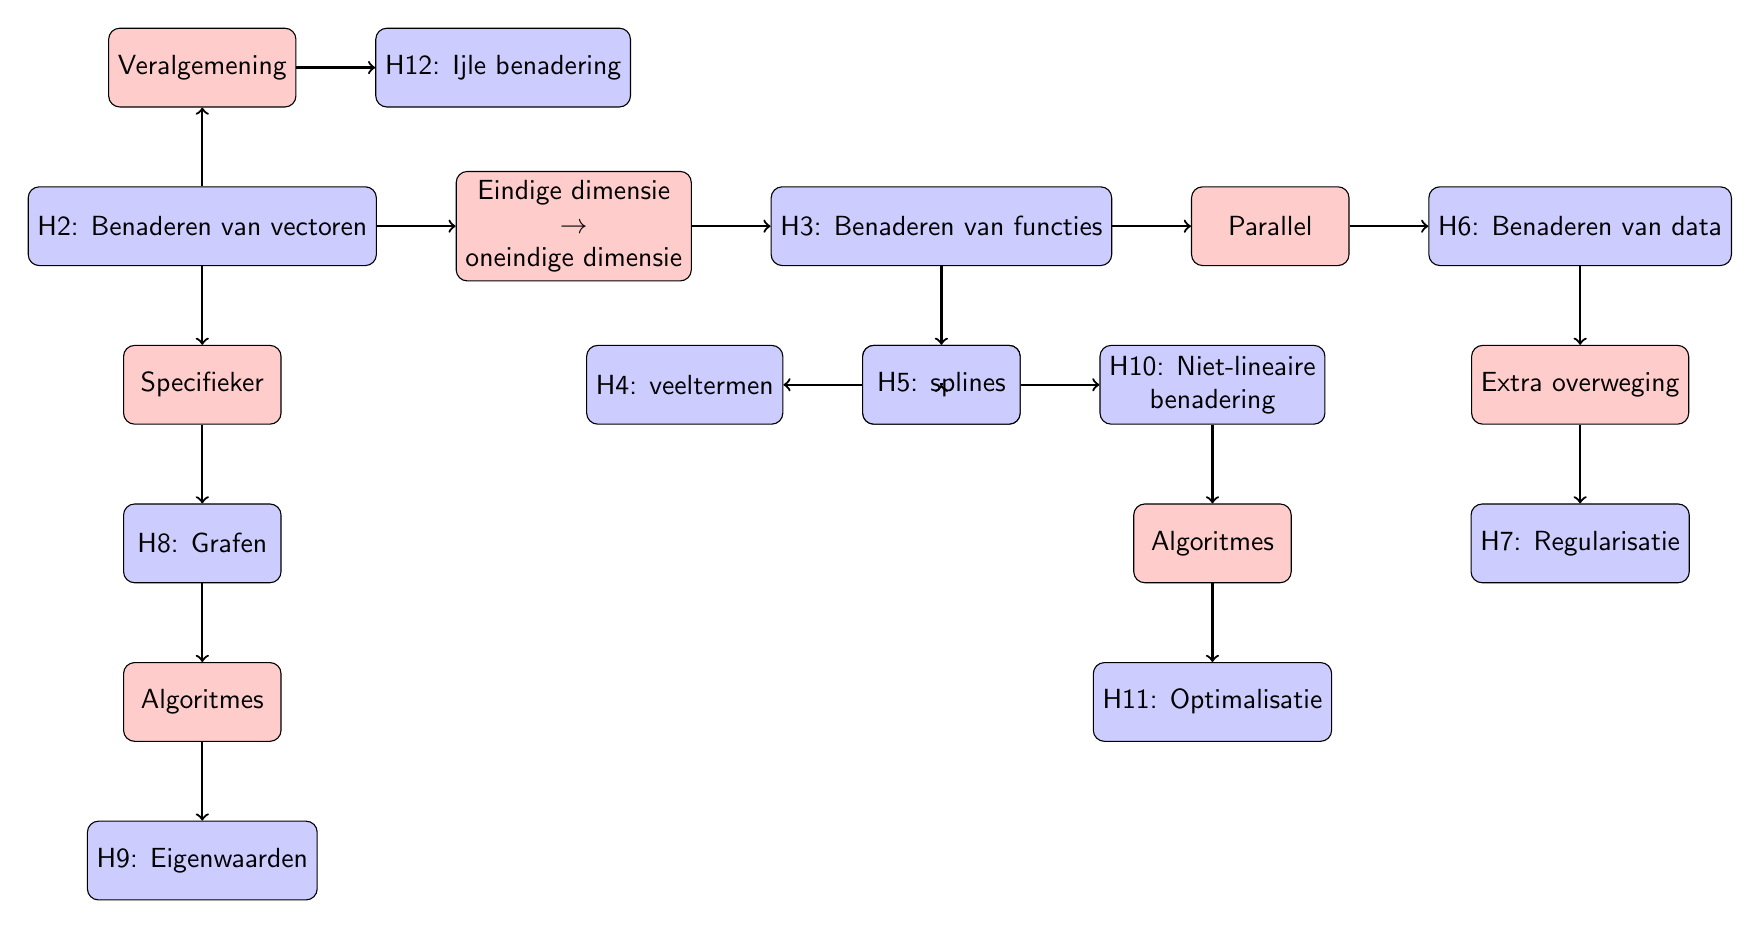
\begin{tikzpicture}[
        node distance=1cm and 1cm,
        every node/.style={font=\sffamily},
        box/.style={draw, rounded corners, minimum width=2cm, minimum height=1cm, align=center},
        bluebox/.style={box, fill=blue!20},
        redbox/.style={box, fill=red!20},
        arrow/.style={->, thick}
    ]
    
    % Nodes
    \node[redbox] (veralgemening) {Veralgemening};
    \node[bluebox, right=of veralgemening] (h12) {H12: Ijle benadering};
    \node[bluebox, below=of veralgemening] (h2) {H2: Benaderen van vectoren};
    \node[redbox, right=of h2] (dimtrans) {Eindige dimensie \\ $\rightarrow$ \\ oneindige dimensie};
    \node[bluebox, right=of dimtrans] (h3) {H3: Benaderen van functies};
    \node[redbox, below=of h2] (specifiek1) {Specifieker};
    \node[bluebox, below=of specifiek1] (h8) {H8: Grafen};
    \node[redbox, below=of h8] (alg1) {Algoritmes};
    \node[bluebox, below=of alg1] (h9) {H9: Eigenwaarden};
    \node[redbox, below=of h3] (specifiek2) {Specifieker};
    \node[bluebox, left=of specifiek2] (h4) {H4: veeltermen};
    \node[bluebox, right=of h4] (h5) {H5: splines};
    \node[bluebox, right=of h5] (h10) {H10: Niet-lineaire \\ benadering};
    \node[redbox, below=of h10] (alg2) {Algoritmes};
    \node[bluebox, below=of alg2] (h11) {H11: Optimalisatie};
    \node[redbox, right=of h3] (parallel) {Parallel};
    \node[bluebox, right=of parallel] (h6) {H6: Benaderen van data};
    \node[redbox, below=of h6] (extra) {Extra overweging};
    \node[bluebox, below=of extra] (h7) {H7: Regularisatie};
    
    % Arrows
    \draw[arrow] (veralgemening) -- (h12);
    \draw[arrow] (h2) -- (veralgemening);
    \draw[arrow] (h2) -- (dimtrans);
    \draw[arrow] (dimtrans) -- (h3);
    \draw[arrow] (h3) -- (parallel);
    \draw[arrow] (parallel) -- (h6);
    \draw[arrow] (h6) -- (extra);
    \draw[arrow] (extra) -- (h7);
    \draw[arrow] (h2) -- (specifiek1);
    \draw[arrow] (specifiek1) -- (h8);
    \draw[arrow] (h8) -- (alg1);
    \draw[arrow] (alg1) -- (h9);
    \draw[arrow] (h3) -- (specifiek2);
    \draw[arrow] (specifiek2) -- (h4);
    \draw[arrow] (specifiek2) -- (h5);
    \draw[arrow] (h5) -- (h10);
    \draw[arrow] (h10) -- (alg2);
    \draw[arrow] (alg2) -- (h11);
    
    \end{tikzpicture}
\end{sidewaysfigure}

\end{document}